\documentclass[bwprint]{gmcmthesis}
\usepackage{amsmath}
\usepackage{multirow}
\usepackage{threeparttable}
\usepackage{pifont}
\usepackage{caption}
\usepackage{subcaption}
\numberwithin{figure}{section}
\renewcommand{\thefigure}{\arabic{section}-\arabic{figure}} 
\newcommand{\upcite}[1]{\textsuperscript{\textsuperscript{\cite{#1}}}}
% \documentclass[withoutpreface,bwprint]{cumcmthesis}
% 去掉封面与编号页

\title{中国研究生数学建模竞赛论文标题}
\baominghao{No.21104870023} %参赛队号
\schoolname{华中科技大学}%学校名称
\membera{张智璐} %队员A
\memberb{钱以骞} %队员B
\memberc{周鑫宜} %队员C
\begin{document}
 \maketitle
 \begin{abstract}
空气污染是环境工程领域与大气科学领域的一个关键研究问题,也与人类的日常生活密切相关。根据污染防治的实践表明,研究污染物与不同气象因素之间的联系,并由此建立空气质量预报模型,提前获知可能发生的大气污染过程并采取相应控制措施,是减少大气污染对人体健康和环境等造成的危害,提高环境空气质量的有效方法之一。传统的预测模型WRF-CMAQ的预测精度有限,因此,结合实测数据对WRF-CMAQ模型进行改进,建立出更加准确的模型是一件非常重要的任务。

针对问题一,我们学习了空气污染指数AQI的计算方式,设计快速计算AQI指数算法,并通过Python语言和pandas等库处理整张表格的数据。将数据处理完成之后,从中提取出2020年8月25日至2020年8月28日每日实测的AQI和首要污染物,并将结果表放入正文中。

对于问题二,本文将气象条件分为3类:对污染物浓度有较显著单向影响类,对污染物浓度有较显著双向影响类,对污染物浓度无显著影响类。首先使用Python语言对附件1中“监测点A逐小时污染物浓度与气象实测数据”表格进行数据处理。对于表格中缺失的数据,采用线性插值法填补缺失的数据。填补完缺失的数据之后,计算出每小时对应的AQI指数以及首要污染物,并对变量进行标准化。由于本题需要根据对污染物浓度的影响程度,对气象条件进行合理分类,因此我们自定义变量AP表示各个污染物浓度对环境恶劣程度的影响,将AP值视作污染物浓度的代表变量。之后,使用SPSS统计软件,对AQI以及标准化之后的污染物浓度变量进行Pearson相关分析,并通过Critic赋权法初步得到AP变量与各污染物变量的权重值。接着,根据各污染物成为首要污染物的比例对初步得到的AP变量权重值进行调整,得到最终AP变量与各污染物变量的权重值。然后对AP变量与各气象因素进行Pearson相关分析,并通过曲线拟合,得到AP变量与各气象因素大致的函数关系,将函数结果可视化进行解释。最后,将5种气象因素分别归类于上述三类之中,并进行简单解释。

对于问题三,本文提出一种基于LSTM的预训练模型,首先预处理逐小时实测数据,保证数据连续,并对每一列进行归一化处理,然后以每小时的6个污染物浓度和5个气象条件作为该小时的特征。从day1的8:00开始,一直取到day3的7:00作为一个时间序列,这个序列的长度为72小时,特征维度是11维,将其输入到3层的LSTM中预测接下来3天,即day3,day4,day5的每日各污染物的平均浓度,即输出是6*3=18维。计算预测出来的3天污染物浓度的MSE并求和,以此作为损失函数训练模型,由此可以通过逐小时的实测数据得到一个预训练模型。接下来需要结合一次预报的数据进行微调,将逐小时实测数据的日期与一次预报对齐,然后仍然是按照前面所述划分出72小时的实测样本时间序列,并将其输入到之前训练好的LSTM模型中,得到最好一个LSTM的隐藏层输出h_t。同时对一次预报数据求出day1,day2,day3预报模型运行得到各数据的平均,将这3天的平均一次预报数据与h_t进行串联经过一个SVM与要预测的未来3天的18维特征相连。同样使用预测的18个污染物浓度与真实污染物浓度的MSE作为损失函数训练第二阶段的模型。

对于问题四,此时我们仍然考虑实验问题三中提到的模型进行预测,但为了使得模型考虑到其他3个监测点的特征,我们考虑同时输入4个监测点的序列,划分时间序列的方法同前面问题三所述,此时将得到一个4×72×11的矩阵,对其进行转置我们得到一个72×4×11的矩阵,也就是在时间序列的每个时刻我们会得到4倍于之前的特征,考虑到减少参数与降维,我们选择对每个时刻使用一个4×1的卷积核进行卷积,经过72个4×1的卷积核的卷积,我们将重新得到72×11维的时间序列,这就与问题三的情况一致了,接下来我们可以继续LSTM预训练模型。同时该卷积核也应用在第二阶段中对来自4个监测点输入的一次预报特征,经过卷积操作降维我们可以继续使用之前的模型进行预测。





\keywords{大气污染物,气象条件,线性插值,Pearson相关系数分析,CRITIC赋值法,LSTM神经网络}%{针对具体的问题列一到两个关键字\quad  建模算法列出\quad }
\end{abstract}

%\pagestyle{plain}

%目录
\tableofcontents
\newpage

\section{问题重述}
\subsection{问题背景}
环境空气污染能够对人类、动植物及产生较大的影响和危害。建立空气质量预报模型,提前预报大气污染状况能够支撑政府制定防治策略,提醒公众提前防范,减少自身暴露,减轻污染。

WRF-CMAQ模拟体系(以下简称WRF-CMAQ模型)是在 “一个大气” 理论的指导下,以WRF中尺度数值天气预报系统为依托,充分考虑了大气污染过程中水平传输、垂直传输、扩散过程、源排放、化学反应和去除过程等对污染物浓度的影响,将复杂空气污染状况进行综合处理\upcite{ref1}。WRF和CMAQ的结构如图\ref{fig1-1}和图\ref{fig1-2}所示。
\begin{figure}[!h]
	\centering
	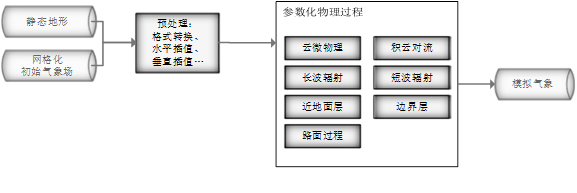
\includegraphics[width=.7\textwidth]{figures//fig1-1.png}
	\caption{中尺度数值天气预报系统WRF结构\upcite{ref2}}
	\label{fig1-1}
\end{figure}
\begin{figure}[!h]
	\centering
	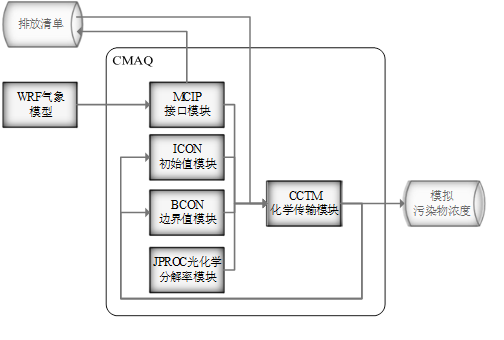
\includegraphics[width=.7\textwidth]{figures//fig1-2.png}
	\caption{空气质量预测与评估系统CMAQ结构\upcite{ref3}}
	\label{fig1-2}
\end{figure}

CMAQ是一种三维欧拉大气化学与传输模拟系统,经由对污染物变化过程的模拟得到具体时间点或时间段的预报结果,但由于模拟的气象场和排放清单的不确定性,同时还存在包括臭氧在内生成机理不完全明晰的污染物的存在,WRF-CMAQ预报模型的结果并不理想。为提高预报准确性,一种可行办法是在WRF-CMAQ等一次模型模拟结果的基础上,结合更多的数据源进行二次建模。二次模型与WRF-CMAQ模型关系如图\ref{fig1-3}所示。其中,由于气象条件对空气质量影响很大(例如湿度降低有利于臭氧的生成),且污染物浓度实测数据的变化情况对空气质量预报具有一定参考价值,因此实测数据源参考空气质量监测点获得的气象数据。
\begin{figure}[!h]
	\centering
	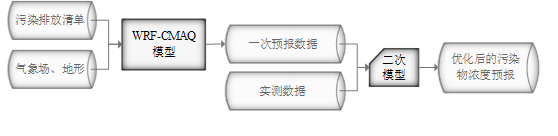
\includegraphics[width=.7\textwidth]{figures//fig1-3.png}
	\caption{空气质量预测与评估系统CMAQ结构}
	\label{fig1-3}
\end{figure}

\subsection{问题提出}
\textbf{问题1}使用附件1数据,计算监测点A从2020年8月25日到8月28日每天实测的AQI和首要污染物。并将结果按照表\ref{tab:table1-1}格式放于正文中
\begin{table}[h!]
	\caption{AQI计算结果表}\label{tab:table1-1}
	\begin{center}
		\begin{tabular}{|c|c|c|c|}
			\hline
			\multirow{2}{*}{检测日期}&\multirow{2}{*}{地点}&\multicolumn{2}{|c|}{AQI计算} \\
			\cline{3-4}
			& &AQI&首要污染物\\
			\hline
			2020/8/25&监测点A&&\\
			\hline
			2020/8/26&监测点A&&\\
			\hline
			2020/8/27&监测点A&&\\
			\hline
			2020/8/28&监测点A&&\\
			\hline
		\end{tabular}
	\end{center}
\end{table}

\textbf{问题2}使用附件1中的数据,根据对污染物浓度的影响程度,对气象条件进行合理分类,并阐述各类气象条件的特征。


\textbf{问题3}使用附件1和2的数据,建立适用3个监测点(忽略彼此影响)的二次预报数学模型,预测未来3天6种污染物浓度,要求预测结果AQI最大相对误差尽量小,首要污染物预测准确度尽量高。并用该模型预测ABC的2021年7月13到7月15的污染物浓度,计算AQI和首要污染物。将结果按照表\ref{tab:table1-2}的格式放于正文中
\begin{table}[h!]
	\caption{AQI计算结果表}\label{tab:table1-2}
	\begin{center}
	\resizebox{.95\columnwidth}{!}{
		\begin{tabular}{|c|c|c|c|c|c|c|c|c|c|}
			\hline
			\multirow{2}{*}{预报日期}&\multirow{2}{*}{地点}&\multicolumn{8}{|c|}{二次模型日值预测} \\
			\cline{3-10}
			& &SO2(μg/m³)&NO2(μg/m³)&PM10(μg/m³)&PM2.5(μg/m³)&O3最大八小时滑动平均(μg/m³)&CO(mg/m³)&AQI&首要污染物\\
			\hline
			2020/7/13&监测点A&&&&&&&&\\
			\hline
			2020/7/14&监测点A&&&&&&&&\\
			\hline
			2020/7/15&监测点A&&&&&&&&\\
			\hline
		\end{tabular}
	}
	\end{center}
\end{table}


\textbf{问题4}使用附件1和3数据建立区域协同预报模型,包含A,A1,A2,A3四个监测点。要求预测结果AQI最大相对误差尽量小,首要污染物预测准确度尽量高。使用该协同预报模型预测监测点A、A1、A2、A3在2021年7月13日至7月15日的污染物浓度,计算AQI和首要污染物。将结果按照表\ref{tab:table1-2}的格式放于正文中。并根据模型预测结果讨论协同预报模型是否能提升准确度。

\section{背景阐述、模型合理假设以及符号说明}
\subsection{背景阐述}
在该问题中,涉及到很多与大气科学领域有关的背景知识,在本节中对部分背景信息进行简单的阐述。
以下分别介绍每种气象条件因素的定义:
\begin{itemize}
	\item 温度是表示物体冷热程度的物理量,微观上来讲是物体分子热运动的剧烈程度。温度只能通过物体随温度变化的某些特性来间接测量,而用来量度物体温度数值的标尺叫温标。在本文中,使用的温标为摄氏温标(°C)。本文中,将该变量简称为T。
	\item 比湿是空气中的水汽质量在混合空气中的质量占比,即
	$$\rm H≡\frac{m_v}{m_v+m_a}$$
	式中,H为比湿,无量纲;$\rm m_v$为空气中的水汽质量,单位:kg;$\rm m_a$为干空气质量,单位:kg。在本文中将该变量简称为H。
	\item 气压是作用在单位面积上的大气压力,即在数值上等于单位面积上向上延伸到大气上界的垂直空气柱所受到的重力。在本文中,使用单位为MPa, 1MPa = 1000000pa。将该变量简称为P。
	\item 风速是指空气相对于地球某一固定地点的运动速率,本文中使用的单位是m/s,1m/s=3.6km/h。本文将该变量简称为WS。
	\item 风向是指风的来向,本题用角度表示。定义自正北方向至监测点的风向为0°风向,以顺时针旋转角(单位:°)为正值记录风向。例如,风自正东方向至监测点时,记录此时段风向为90°。本文将该变量简称为WD。
\end{itemize}

以下介绍一些气象科学相关名词的定义:
\begin{itemize}
	\item 污染天气:
	空气质量污染天气指当日空气质量评级达到“轻度污染”或更高等级的天气。在本题中,空气质量等级是以空气质量指数(Air Quality Index, AQI)为指标进行划分,当某日AQI超过100时,视当日天气为污染天气。
	\item 一次污染物与二次污染物:
	一次污染物是指直接从污染源排到大气中的原始污染物质,如硫氧化物(SOx)、氮氧化物(NOx)等。二次污染物则是指由一次污染物与大气中已有组分或几种一次污染物之间经过一系列化学或光化学反应而生成的与一次污染物性质不同的新污染物质,如臭氧、硫酸盐、硝酸盐、有机颗粒物等。
	\item 一种近地面臭氧污染形成机制:
	图\ref{fig2-1}为近地面臭氧污染形成的一种机制。该机制中,自由基循环和NOx循环相互耦合作用,使NO不断转化为NO2,NO2的光解使O3逐渐积累,导致污染的产生。总的来说,臭氧污染形成过程受到多种一次污染物因素\upcite{ref3}及光照强度等气象因素的影响。
	\item 臭氧(O3)最大8小时滑动平均:
	指一个自然日内8时至24时的所有8小时滑动平均浓度中的最大值,其中8小时滑动平均值指连续8小时平均浓度的算术平均值。其计算公式如下:
	$$
		\rm C_{O_3}=max_T(t=8,9,…,24)⁡{\frac{1}{8}\sum_{i=t-7}^{t}{c_t}}
	$$
	其中$\rm c_t$为臭氧在某日t-1时至t时的平均污染物浓度。
	\item 预测时间/监测时间:
	预测时间/监测时间是逐小时一次预报数据/实测数据的时间点标记,对应的气象及污染物浓度数据为该时间点起一小时内的平均值。以一次预报数据为例,预测时间为“2020/11/04 05:00”的数据行中, SO2浓度为$\rm X μg∕m^3$,表示SO2在2020年11月4日5:00-6:00的平均浓度预测值为$\rm X μg∕m^3$。
	\item 边界层高度:
	附件中的边界层高度是指大气边界层顶部距地面的高度,单位:m。其中,大气边界层是地表与大气进行热量、水汽与空气污染物交换、混合的第一通道,也是气团活动主要场所。边界层上方的自由大气向下流动时,由于无法穿越冠盖逆温层,形成一股向下的压力,使得边界层被压缩,近地污染物较易富集。
	\item 长波辐射/短波辐射/地面太阳能:
	长波辐射、短波辐射和地面太阳能均为与地面吸收太阳光照能量有关的指标。其中,长波辐射指地面向宇宙辐射长波的地表能通量,短波辐射指地面吸收的太阳能短波辐射的地表能通量,地面太阳能指地面吸收的太阳能所有波长辐射的地表能通量,三者单位:$\rm W/m^2$。
	\item 感热通量/潜热通量:
	在不发生物体和媒介的相态变化条件下,通过热传导和对流(湍流)所输送的能量称为感热;由物质发生相变而吸收或放出的热能则称为潜热。地面吸收的太阳辐射能会以感热形式及潜热形式释放至大气中,附件中以能通量形式表示这部分感热及潜热。单位:$\rm W/m^2$。。当气温高于地温时,感热通量/潜热通量为负值。
\end{itemize}

\begin{figure}[!h]
	\centering
	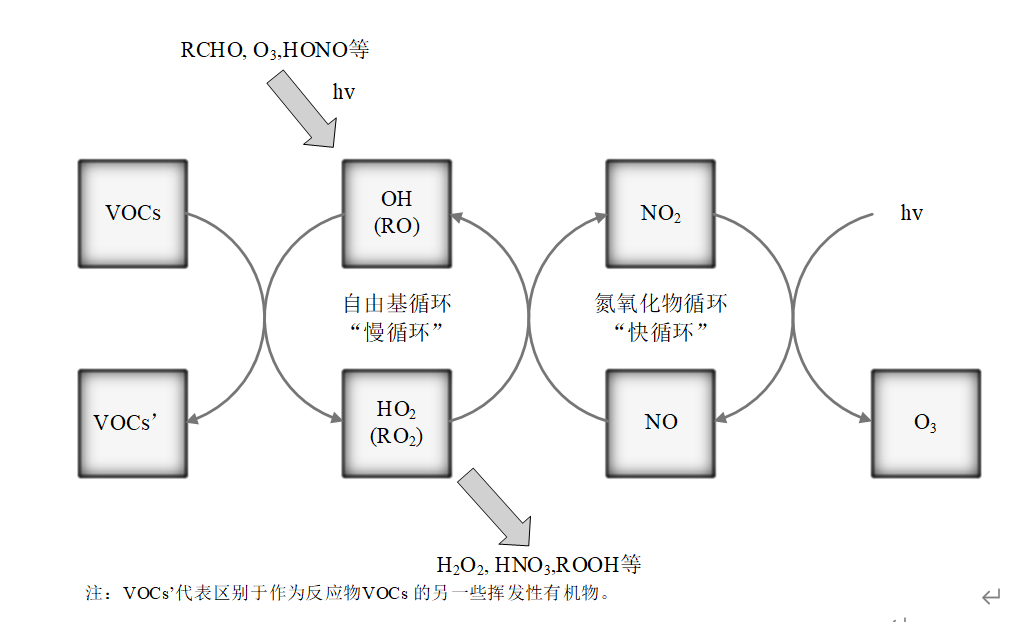
\includegraphics[width=.7\textwidth]{figures//fig2-1.png}
	\caption{一种臭氧与氮氧化物之间相互转化的反应过程\upcite{ref5}}
	\label{fig2-1}
\end{figure}

\subsection{模型合理假设}
a.假设本题涉及到的所有大气科学相关变量(气象条件或是污染物浓度等)在自然界都是连续变量

b.假设各个气象条件因素之间相互独立。

c.假设在连续时间段内,由工业、生活等人类日常行为产生的污染物排放浓度不会发生突变。

d.假设在连续时间段内,气象因素不会发生突变。

e.对于问题3,假设3个监测点的位置较远,忽略其之间的相互影响。

\subsection{符号说明}
对本文中涉及到的符号及其意义如表\ref{tab:table2-1}所示:
\begin{table}[h!]
	\caption{本文涉及到的部分符号说明}\label{tab:table2-1}
	\begin{center}
		\begin{tabular}{|c|c|}
			\hline
			符号&说明\\
			\hline
			T&温度变量\\
			H&比湿变量\\
			P&气压变量\\
			WS&风速变量\\
			WD&风向变量\\
			$\rm ZX$&某个变量的标准化变量\\
			\hline
		\end{tabular}
	\end{center}
\end{table}

注:为了方便论文的阅读,模型涉及到的部分参量符号未在表中一一列举,而是在各表达式后进行解释说明
\section{问题的分析}
\subsection{问题一:通过给定污染物数据计算当日的AQI指数}
\subsubsection{AQI指数计算方式与相关背景}
AQI即为空气质量指数,该数据可用于判别空气质量等级。AQI的计算方式如下:
首先需得到各项污染物的空气质量分指数(IAQI),其计算公式如公式(1)所示:
\begin{equation}
	\rm IAQI_P = \frac{IAQI_{Hi}-IAQI_{Lo}}{BP_{Hi}-BP_{Lo}}*(C_P-BP_{Lo})+IAQI_{Lo}
\end{equation}
式中各符号的含义如下:
\begin{itemize}
	\item $\rm IAQI_P$表示污染物P的空气质量分指数,结果进位取整数
	\item $\rm C_P$表示污染物P的质量浓度值
	\item $\rm BP_{Hi}, BP_{Lo}$表示与$\rm C_P$相近的污染物浓度限值的高位值与低位值
	\item $\rm IAQI_{Hi}, IAQI_{Lo}$表示与$\rm BP_{Hi},BP_{Lo}$对应的空气质量分指数
\end{itemize}

各项污染物项目浓度限值及对应的空气质量分指数级别见表\ref{tab:table4-1}:
\begin{table}[h!]
\caption{空气质量分指数(IAQI)及对应的污染物项目浓度限值}\label{tab:table4-1}
\begin{center}
\begin{threeparttable}
\resizebox{.95\columnwidth}{!}{
\begin{tabular}{|c|c|c|c|c|c|c|c|c|c|c|}
	\hline
	序号&指数或污染物项目&\multicolumn{8}{|c|}{空气质量分指数及对应污染物浓度限值}&单位 \\
	\hline
	0&空气质量分指数(IAQI)&0&50&100&150&200&300&400&500&-\\
	\hline
	1&一氧化碳(CO)24小时平均&0&2&4&14&24&36&48&60&$\rm mg∕m^3$\\
	\hline
	2&二氧化硫(SO2)24小时平均&0&50&150&475&800&1600&2100&2620&\multirow{5}{*}{$\rm μg∕m^3$} \\
	\cline{1-10}
	3&二氧化氮(NO2)24小时平均&0&40&80&180&280&565&750&940& \\
	\cline{1-10}
	4&臭氧(O3)最大8小时滑动平均&0&100&160&215&265&800&-&-& \\
	\cline{1-10}
	5&粒径小于等于10μm颗粒物
	(PM10)24小时平均&0&50&150&250&350&420&500&600& \\
	\cline{1-10}
	6&粒径小于等于2.5μm颗粒物
	(PM2.5)24小时平均&0&35&75&115&150&250&350&500& \\
	\hline
\end{tabular}
}
\begin{tablenotes}
	\footnotesize
	\item[1] 臭氧(O3)最大8小时滑动平均浓度值高于800 $\rm μg∕m^3$的,不再进行其空气质量分指数计算。
	\item[2] 其余污染物浓度高于IAQI=500对应限值时,不再进行其空气质量分指数计算
\end{tablenotes}
\end{threeparttable}      
\end{center}
\end{table}


空气质量指数(AQI)取各分指数中的最大值,即有
\begin{displaymath} 
	\rm AQI = max{IAQI_1,IAQI_2,...,IAQI_n}
\end{displaymath}
式中,$\rm IAQI_1,IAQI_2,IAQI_3,…,IAQI_n$为各污染物项目的分指数。在本题中,对于AQI的计算仅涉及表1提供的六种污染物,因此计算公式如公式(2)所示:
\begin{equation} 
	\rm AQI = max⁡{IAQI_{SO_2},IAQI_{NO_2},IAQI_{PM_10},IAQI_{PM_2.5},IAQI_{O_3},IAQI_CO}
\end{equation}
空气质量等级范围根据AQI数值划分,等级对应的AQI范围见表\ref{tab:table4-2}。
\begin{table}[h!]
	\caption{空气质量等级及对应空气质量指数(AQI)范围}\label{tab:table4-2}
	\begin{center}
		\begin{tabular}{|c|c|c|c|c|c|c|}
			\hline
			空气质量等级&优&良&轻度污染&中度污染&重度污染&严重污染 \\
			\hline
			空气质量指数(AQI)范围&[0,50]&[51,100]&[101,150]&[151,200]&[201,300]&[301,+∞) \\
			\hline
		\end{tabular}
	\end{center}
\end{table}

当AQI小于或等于50(即空气质量评价为“优”)时,称当天无首要污染物;
当AQI大于50时,IAQI最大的污染物为首要污染物。若IAQI最大的污染物为两项或两项以上时,并列为首要污染物
IAQI大于100的污染物为超标污染物。
则求解问题一需要根据附件1中提供的“监测点A逐日污染物浓度数据”表,通过上述方法计算监测点A从2020年8月25日到8月28日每天实测的AQI和首要污染物。
\subsubsection{快速求解AQI指数算法及对应结果}
求解AQI指数的过程非常简单,但是我们为了后期处理的方便性以及增强代码的可重用性,我们采用直接完全处理附件1中的“监测点A逐日污染物浓度数据”表的方式。在得到整个表的结果后,找出题目中的日期范围对应的结果。处理整个表格的流程图如图\ref{fig3-1}所示:
\begin{figure}[!h]
	\centering
	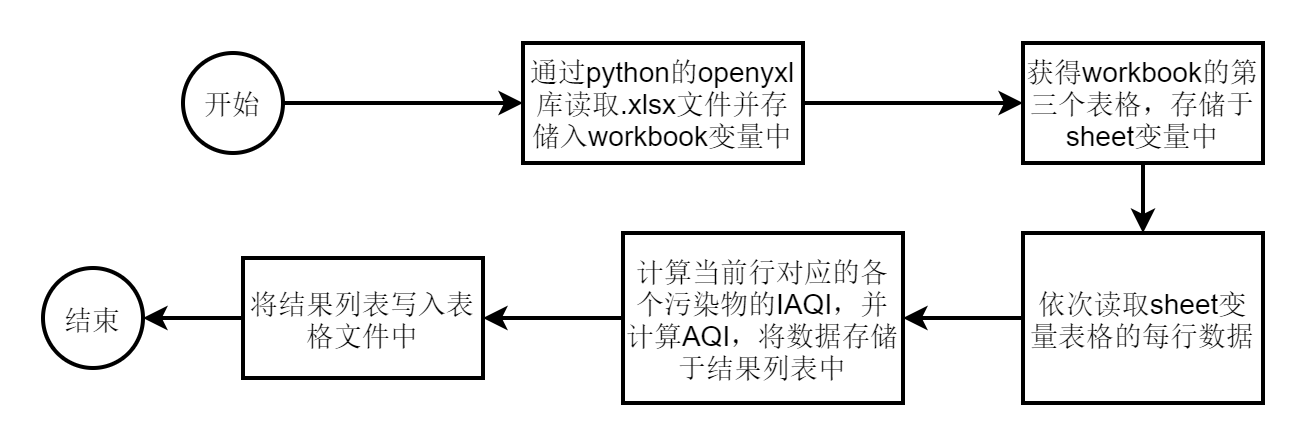
\includegraphics[width=.7\textwidth]{figures//fig3-1.png}
	\caption{完全处理“监测点A逐日污染物浓度数据”表流程图}
	\label{fig3-1}
\end{figure}

计算得到的结果如表\ref{tab:table4-3}所示
\begin{table}[h!]
	\caption{问题一AQI计算结果表}\label{tab:table4-3}
	\begin{center}
		\begin{tabular}{|c|c|c|c|}
			\hline
			\multirow{2}{*}{检测日期}&\multirow{2}{*}{地点}&\multicolumn{2}{|c|}{AQI计算} \\
			\cline{3-4}
			& &AQI&首要污染物\\
			\hline
			2020/8/25&监测点A&60&$\rm O_3$\\
			\hline
			2020/8/26&监测点A&46&无\\
			\hline
			2020/8/27&监测点A&109&$\rm O_3$\\
			\hline
			2020/8/28&监测点A&138&$\rm O_3$\\
			\hline
		\end{tabular}
	\end{center}
\end{table}

\subsection{问题二:根据对污染物浓度的影响程度,对气象条件进行分类}
\subsubsection{问题分析与数据预处理}
根据附件1中“监测点A逐小时污染物浓度与气象实测数据”表的数据,我们可以得到可能对污染物浓度产生影响的气象条件因素有5种:温度,比湿,气压,风速与风向。其具体定义已于章节2中阐述,此处不再赘述。

在污染物排放情况不变的条件下,某一地区的气象条件有利于污染物扩散或沉降时,该地区的AQI会下降,反之会上升。由此分析出,在不同气象条件下的AQI指数可以很好地反应气象条件对污染物浓度的影响。与此同时,也要分别分析6种污染物(CO,NO2,SO2,O3,PM10,PM2.5)在不同气象条件下的浓度变化情况。因此,如何自定义一个变量用于标志各种不同的污染物对环境恶劣程度的影响。分析思路如下:首先计算AQI变量与各个污染物变量的相关性,然后通过主客观集成赋权法得到6种污染物浓度分别对我们最终定义的污染物对环境恶劣程度影响变量(称为AP)的影响权重。再通过各个污染物成为首要污染物的比例,对影响权重进行修正。最后通过相关性分析与插值法建模得到气象因素对AP的影响,我们可以将气象条件因素分为三类:对污染物浓度有较显著单向影响类因素,对污染物浓度有较显著的双向影响因素,对污染物浓度无显著影响因素。对三种类别的解释如下:
\begin{itemize}
	\item 对污染物浓度有较为显著的单向影响因素类别的主要表现为:随着该因素变量值的上升,对AP的影响是单方面的(无论是正相关抑或是负相关),例如随着该因素变量的上升,AP指数不断下降。
	\item 对污染物浓度有较为显著的双向影响因素类别的主要表现为:随着该因素变量值的上升,对AP的影响是双方面的,例如在某个区间内,该因素的上升AP指数的下降,但在另一个区间内,该因素的上升导致AP指数的上升。
	\item 对污染物浓度无显著影响因素类别的主要表现为:随着该因素变量的改变,对AP指数没有显著的影响。
\end{itemize}

在正式建立模型之前,对表格数据进行如下预处理:

(1)填补缺失数据:
由于受监测数据权限及相应监测设备功能等的限制,部分气象指标的实测数据无法获得,因此在表格中存在着部分数据缺失的情况。

由于在章节2中对污染物变量与气象因素变量有不产生突变的合理假设。因此对于插值法,本文采用线性插值的方式,用于填补表格中的缺失数据。线性插值是指插值函数为一次多项式的插值方式,其在插值节点上的插值误差为零。线性插值相比其他插值方式,如抛物线插值,具有简单、方便的特点。线性插值的几何意义即为图\ref{fig3-2}中利用过A点和B点的直线来近似表示原函数。线性插值可以用于近似代替原函数,也可以用于计算得到查表过程中表中缺失的数值。
\begin{figure}[!h]
	\centering
	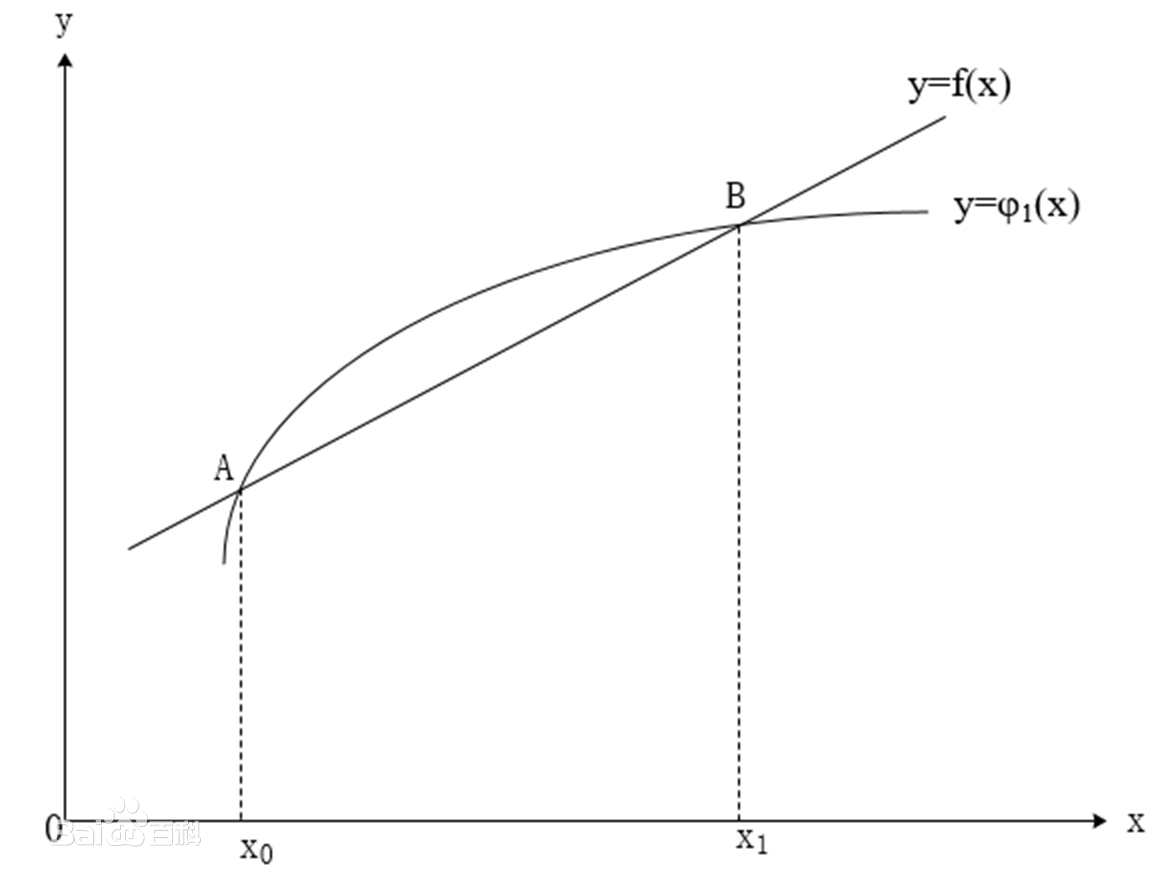
\includegraphics[width=.7\textwidth]{figures//fig3-2.png}
	\caption{线性插值示意图}
	\label{fig3-2}
\end{figure}

如图\ref{fig3-2}所示,设函数$\rm y = f(x)$在$\rm x_0$,$\rm x_1$点的取值分别为$\rm y_0$,$\rm y_1$,求多项式
$$\rm y = φ_1(x) = a_0+a_1x$$
使满足
$$\rm φ_1(x_0) = y_0, φ_1(x1) = y_1 $$
由解析几何易得:
$$\rm y = φ_1(x) = y_0 +\frac{y_1-y_0}{x_1-x_0}(x-x_0)	$$
使用线性插值法可以填补表中的缺失值,并在之后的处理过程中将插入值作为缺失值的替代

(2)通过污染物浓度计算AQI指数:
AQI指数的计算方法在问题一中已经进行阐述,此处不再赘述。对每个小时的污染物浓度数据,都可以计算出其相应的AQI指数。

(3)数据的标准化:
由于数据的量纲不同,我们需要变量数据进行标准化。标准化原始变量数据采用如公式(3)方式:
\begin{equation}
	\rm ZX_i = \frac{X_i-μ}{δ}, μ = \frac{1}{n}\sum_{i=1}^{n}X_i, δ = \sqrt{\frac{1}{n-1}\sum_{i=1}^{n}(X_i-μ)^2}
\end{equation}
将标准化之后AQI,SO3,NO2,O3,PM10,PM2.5,CO变量对应的新变量分别命名为ZAQI,ZSO3,ZNO2,ZO3,ZPM10,ZPM2.5,ZCO。将标准化之后的T,H,P,WS,WD等变量分别命名为ZT,ZH,ZP,ZWS,ZWD

\subsubsection{模型建立、求解与验证}
(1)Person相关系数分析

在本题中,研究变量之间的相关性采用Pearson相关系数进行分析。Pearson相关系数是用来衡量两个数据集合是否在一条线上面,它用来衡量定距变量间的线性关系的一种评价指标。当两个变量都是正态连续变量,而且两者之间呈线性关系时,表现这两个变量之间相关程度用积差相关系数,主要有Pearson简单相关系数。
其计算方式如公式(4)所示:
\begin{equation}
	\rm r = \frac{N\sum{x_iy_i}-\sum{x_i}\sum{y_i}}{\sqrt{N\sum{x_i^2}-(\sum{x_i})^2}\sqrt{N\sum{y_i^2}-(\sum{y_i})^2}}
\end{equation}
Pearson相关系数衡量的是线性相关关系。若r=0,只能说x与y之间无线性相关关系,不能说无相关关系。相关系数的绝对值越大,相关性越强:相关系数越接近于1或-1,相关度越强,相关系数越接近于0,相关度越弱。
此处使用Python和SPSS统计软件,分析ZAQI,ZNO2,ZSO3,ZO3,ZCO,ZPM10,ZPM2.5之间的Person相关性的步骤如下:
\ding{172} 使用Python对Excel数据进行处理,通过线性插值填补缺失值,并计算出每一行对应的AQI指数

\ding{173} 使用SPSS软件导入Excel数据

\ding{174} 通过SPSS软件,点击分析→描述统计→描述,选择AQI等12个变量,并将标准化之后的变量另存为变量ZAQI等变量。

\ding{175} 通过SPSS软件,点击相关→双变量,选择ZAQI、ZCO等6个变量,得到其Pearson相关系数矩阵

其相关系数矩阵如图\ref{fig3-3}所示:
\begin{figure}[!h]
	\centering
	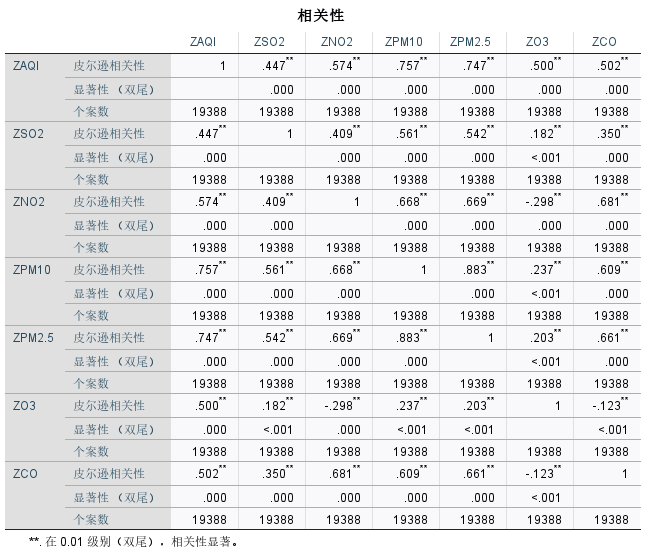
\includegraphics[width=.7\textwidth]{figures//fig3-3.png}
	\caption{ZAQI变量Person相关矩阵示意图}
	\label{fig3-3}
\end{figure}

(2)通过Critic赋权法以及首要污染物占比调整确定AP表达式

确定某种变量的权重主要有两大类:一类是主观权重赋值法,例如AHP、专家评分法等;还有一类就是客观权重赋权法,比较典型的就是Critic赋值法。
Critic赋值法以两个基本概念为基础:一是对比强度,借鉴标准离差法的思想,认为若同一指标的所有评价指数差别越大,即标准差越大,则所蕴含的信息量越大;二是评价指标之间的冲突性,指标之间的冲突性是以指标之间的相关系数为基础,如两个指标之间具有较强的正相关,说明两个指标冲突性较低。第j个指标与其它指标的冲突性的量化指标$\rm \sum_{i=1}^{n}(1-r_{ij})$,其中$\rm r_{ij}$评价指标i和j之间的相关系数。各个指标的客观权重确定就是以对比强度和冲突性来综合衡量的。设$\rm C_j$表示第j个评价指标所包告的信息量。$\rm C_j$的计算式如下:
$$
\rm C_j=δ_j \sum_{i=1}^{n}1-r_{ij}     
$$
其中n为同一指标的评价数量。一般地,$\rm C_j$越大,第j个评价指标所包含的信息量越大,则该指标的相对重要性也就越大。

设$\rm W_j$为第j个指标的客观权重。$\rm W_j$的计算公式:$\rm W_j=\frac{C_j}{\sum_{i=1}^{m}C_i} $(m为所有指标的数量)
通过Critic赋权法可以计算出对于自定义因变量AP关于ZNO2等变量的权重,最后通过加权求和的方式得到最终的计算公式:
\begin{equation}
	\rm AP = \sum_{i=1}^{n}W_iZX_i
\end{equation}
该过程的数学解释为:通过计算AQI与6中污染物的相关性,反映了不同的污染物,其浓度变化对AQI变化的影响,对AQI变化影响较大的污染物,赋予更高的权重。
通过Python程序,计算出的权重表如表\ref{tab:table4-4}所示:(精确至小数点后三位)
\begin{table}[h!]
	\caption{AP权重计算结果表}\label{tab:table4-4}
	\begin{center}
		\begin{tabular}{|c|c|c|c|c|c|}
			\hline
			变量名&权重&变量名&权重&变量名&权重 \\
			\hline
			ZSO2&0.127&ZNO2&0.163&ZPM10&0.215 \\
			\hline
			ZPM2.5&0.212&ZO3&0.142&ZCO& 0.142\\
			\hline
		\end{tabular}
	\end{center}
\end{table}

但是主观上认为直接使用该权重有一定的误差,因为在对监测点A逐小时污染数据处理计算AQI值和首要污染物之后,发现污染物CO和SO2成为首要污染物的比例非常低,甚至没有任何一个小时其SO2污染物为首要污染物。因此希望引入各个污染物成为首要污染物的比例,来修正各个变量的权重值。分析认为:在最终的权重表中,相关系数仍然应当占据更大的权重比例,但与此同时,各个污染物成为首要污染物的比例也是不可忽视的,分析后人为确定两者的权重分别为0.6与0.4。得到如下计算方式:
\begin{equation*}
	\rm newW_i = 0.6*W_i+0.4*P_i,P_i = \frac{T_i}{\sum{T_i}}
\end{equation*}
其中$\rm T_i$表示第i中污染物成为首要污染物的次数

进行修正之后得到的权重表如表\ref{tab:table4-5}所示:
\begin{table}[h!]
	\caption{AP权重计算结果表}\label{tab:table4-5}
	\begin{center}
		\begin{tabular}{|c|c|c|c|c|c|}
			\hline
			变量名&权重&变量名&权重&变量名&权重 \\
			\hline
			ZSO2&0.076&ZNO2&0.260&ZPM10&0.226 \\
			\hline
			ZPM2.5&0.165&ZO3&0.182&ZCO&0.091\\
			\hline
		\end{tabular}
	\end{center}
\end{table}

则有AP计算公式如下所示
\begin{equation*}
	\rm AP = 0.076*ZSO_2+0.260*ZNO_2+0.226*ZPM_{10}+0.165*ZPM_{2.5}+0.182*ZO_3+0.091*ZCO
\end{equation*}

(3)分析AP与气象条件因素的相关性并统计AP在某种气象条件下的平均值变化率
	通过SPSS软件直接定义新变量AP,通过定义计算表达式计算出AP的取值。然后对变量AP,GT,GH,GP,GWS,GWD等变量进行相关性分析,得到相关性矩阵如图\ref{fig3-4}所示:
	\begin{figure}[!h]
		\centering
		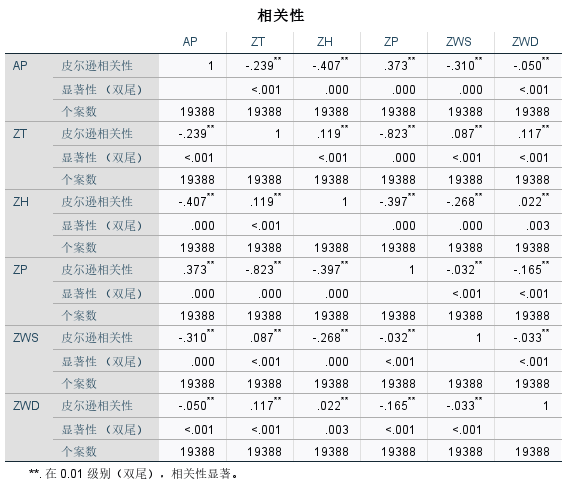
\includegraphics[width=.7\textwidth]{figures//fig3-4.png}
		\caption{变量AP的Person相关系数矩阵}
		\label{fig3-4}
	\end{figure}
	
	从图\ref{fig3-4}中各个变量对应的Pearson相关系数,我们可以看出:变量ZWD(即标准化之后的风速变量)对AP变量的影响比较小,其余因素对变量AP的取值都有较大影响,可视化统计AP变量与各个气象因素条件如下:
	
	\ding{172} 可视化统计AP变量与风速变量WS之间的关系:
	
	将“监测点A逐小时污染物浓度与气象实测数据”表中每小时风速变量WS与对应计算出的AP变量值进行一一对应,并求出每一个特定的WS取值下对应AP变量取值的均值。并将结果绘制为折线图,其结果如图\ref{fig3-5}所示:
	\begin{figure}[!h]
		\centering
		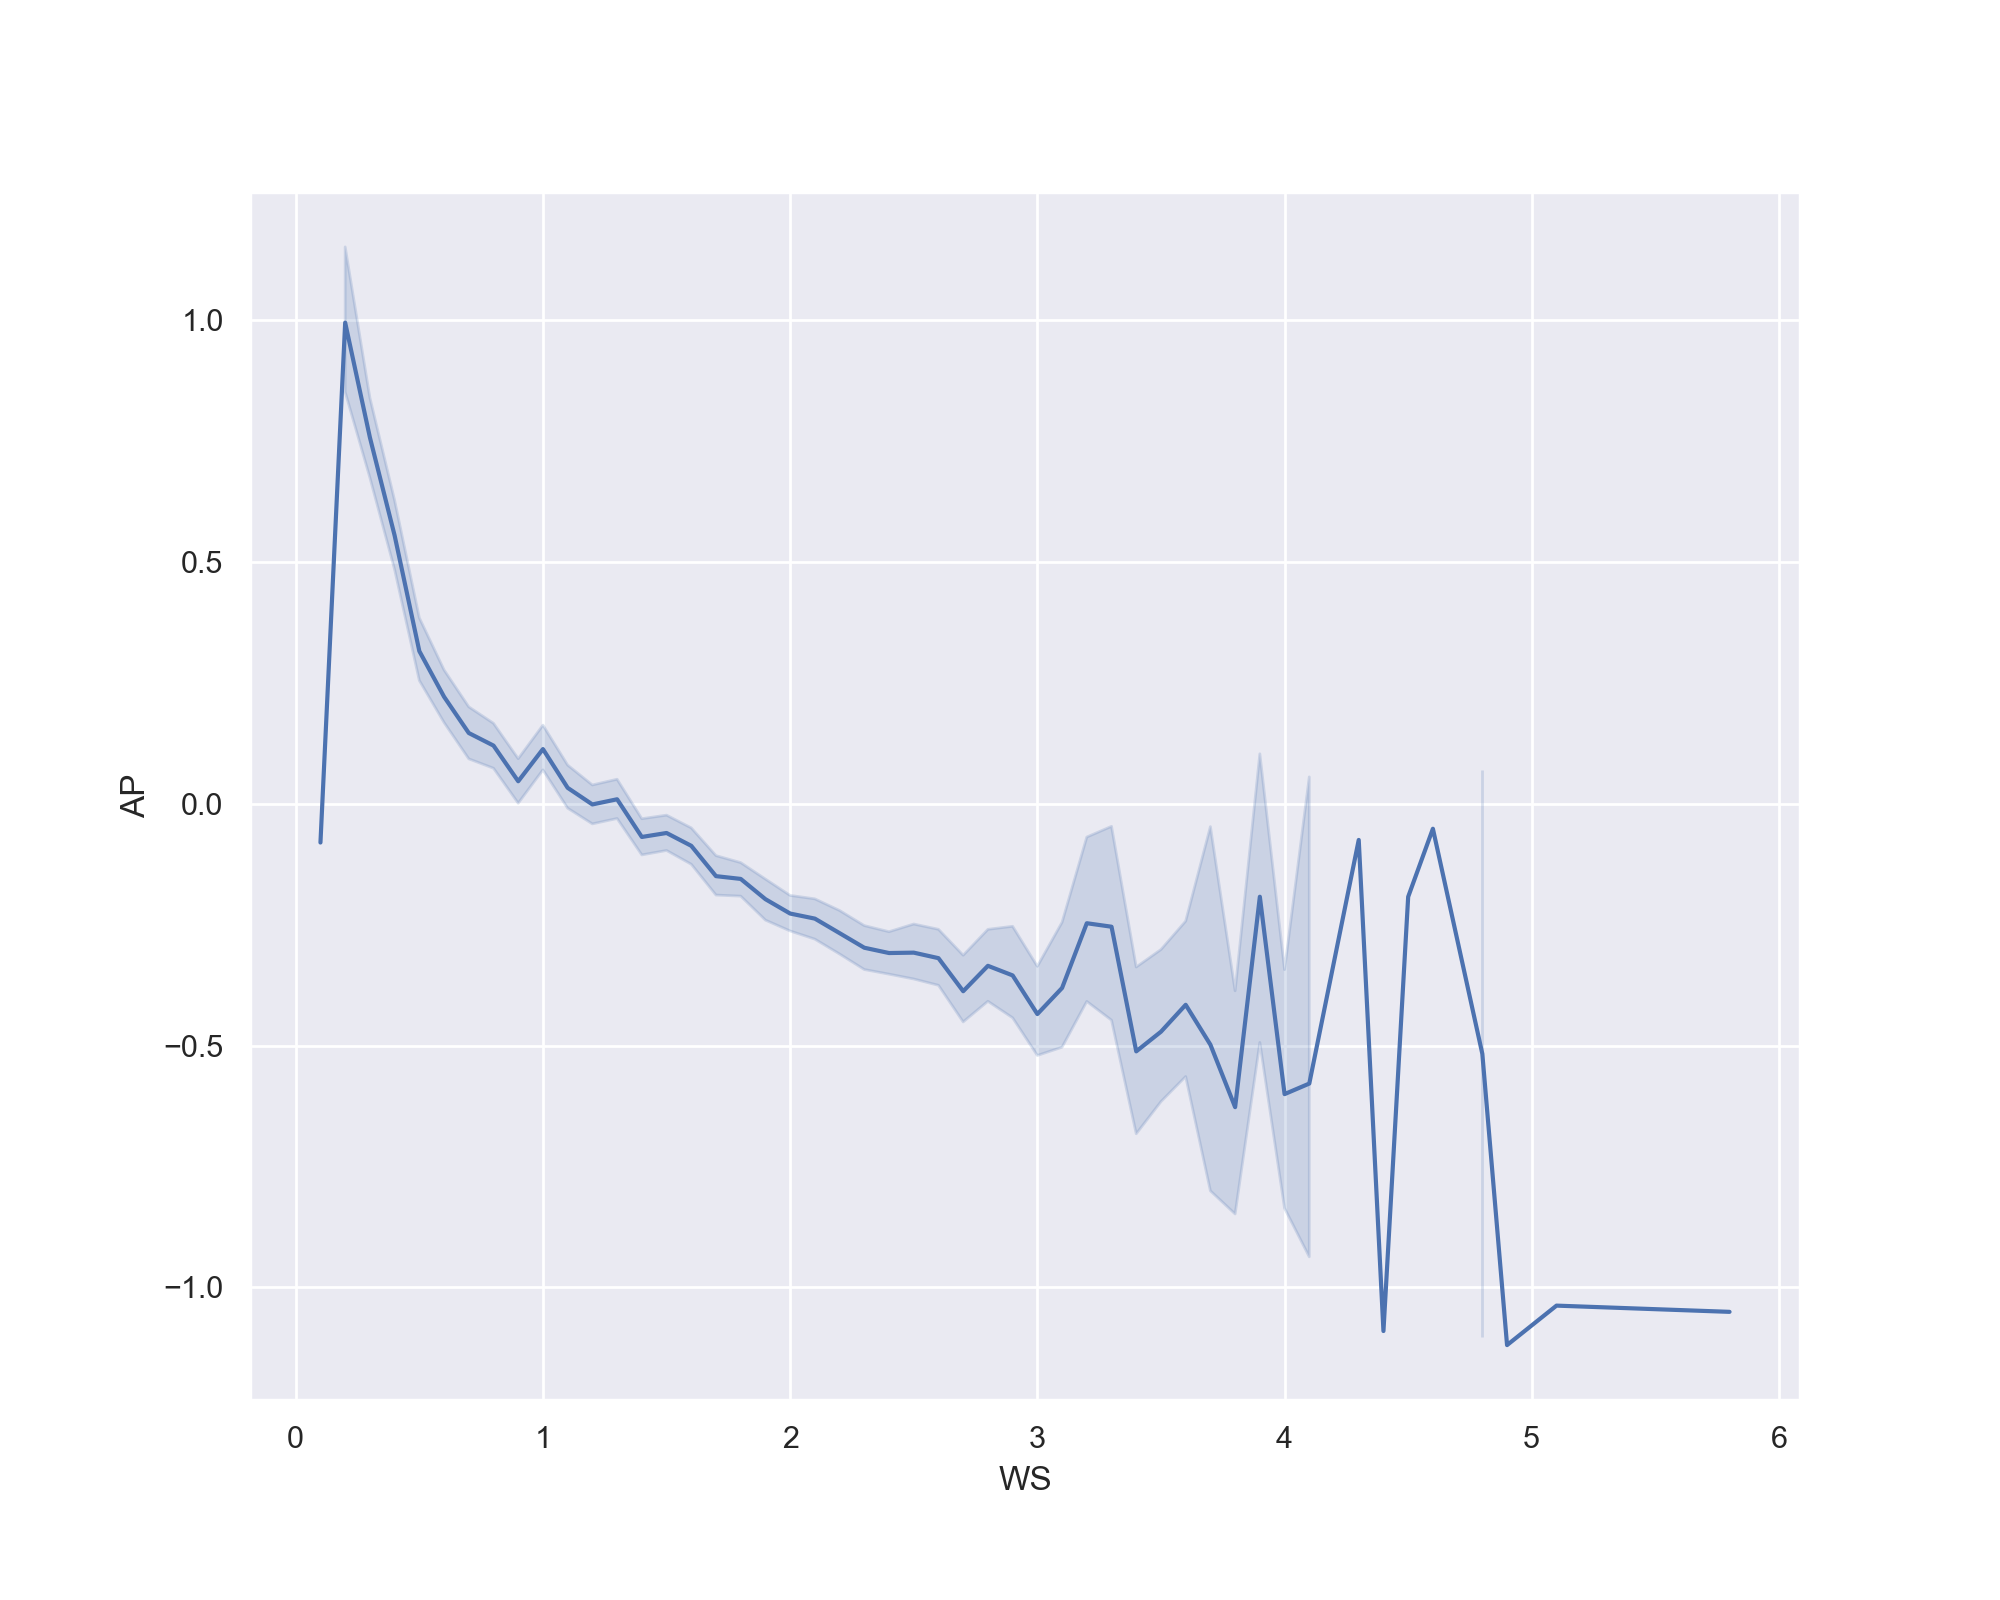
\includegraphics[width=.7\textwidth]{figures//fig_WS.png}
		\caption{变量AP与风速变量WS的折线图}
		\label{fig3-5}
	\end{figure}

虽然图中折线的震荡性非常强,但是仍然可以大致看出随着风速变量WS的上升,对应的AP变量呈现下降的趋势。为了研究AP变量随变量WS的变化趋势,使用曲线拟合的方式对变量的变化趋势进行拟合。

曲线拟合的定义如下:用连续曲线近似地刻画或比拟平面上离散点组所表示的坐标之间的函数关系的一种数据处理方法。用解析表达式逼近离散数据的一种方法。在科学实验或社会活动中,通过实验或观测得到量x与y的一组数据对$\rm (x_i,y_i)(i=1,2,...,m)$,其中各$\rm x_i$是彼此不同的 。人们希望用一类与数据的背景材料规律相适应的解析表达式,$\rm y=f(x,c)$来反映量x与y之间的依赖关系,即在一定意义下“最佳”地逼近或拟合已知数据。$\rm f(x,c)$常称作拟合模型 ,式中$\rm c=(c_1,c_2,...,cn)$是一些待定参数。当c在f中线性出现时,称为线性模型,否则称为非线性模型。有许多衡量拟合优度的标准,最常用的一种做法是选择参数c使得拟合模型与实际观测值在各点的残差(或离差)$\rm e_k=y_k-f(x_k,c)$的加权平方和达到最小,此时所求曲线称作在加权最小二乘意义下对数据的拟合曲线。有许多求解拟合曲线的成功方法,对于线性模型一般通过建立和求解方程组来确定参数,从而求得拟合曲线。至于非线性模型,则要借助求解非线性方程组或用最优化方法求得所需参数才能得到拟合曲线,有时称之为非线性最小二乘拟合。

在Python中,numpy库可以用于曲线拟合。调用numpy库对自变量WS和因变量WT进行曲线拟合,所得结果如图\ref{fig3-6}所示:
\begin{figure}[!h]
	\centering
	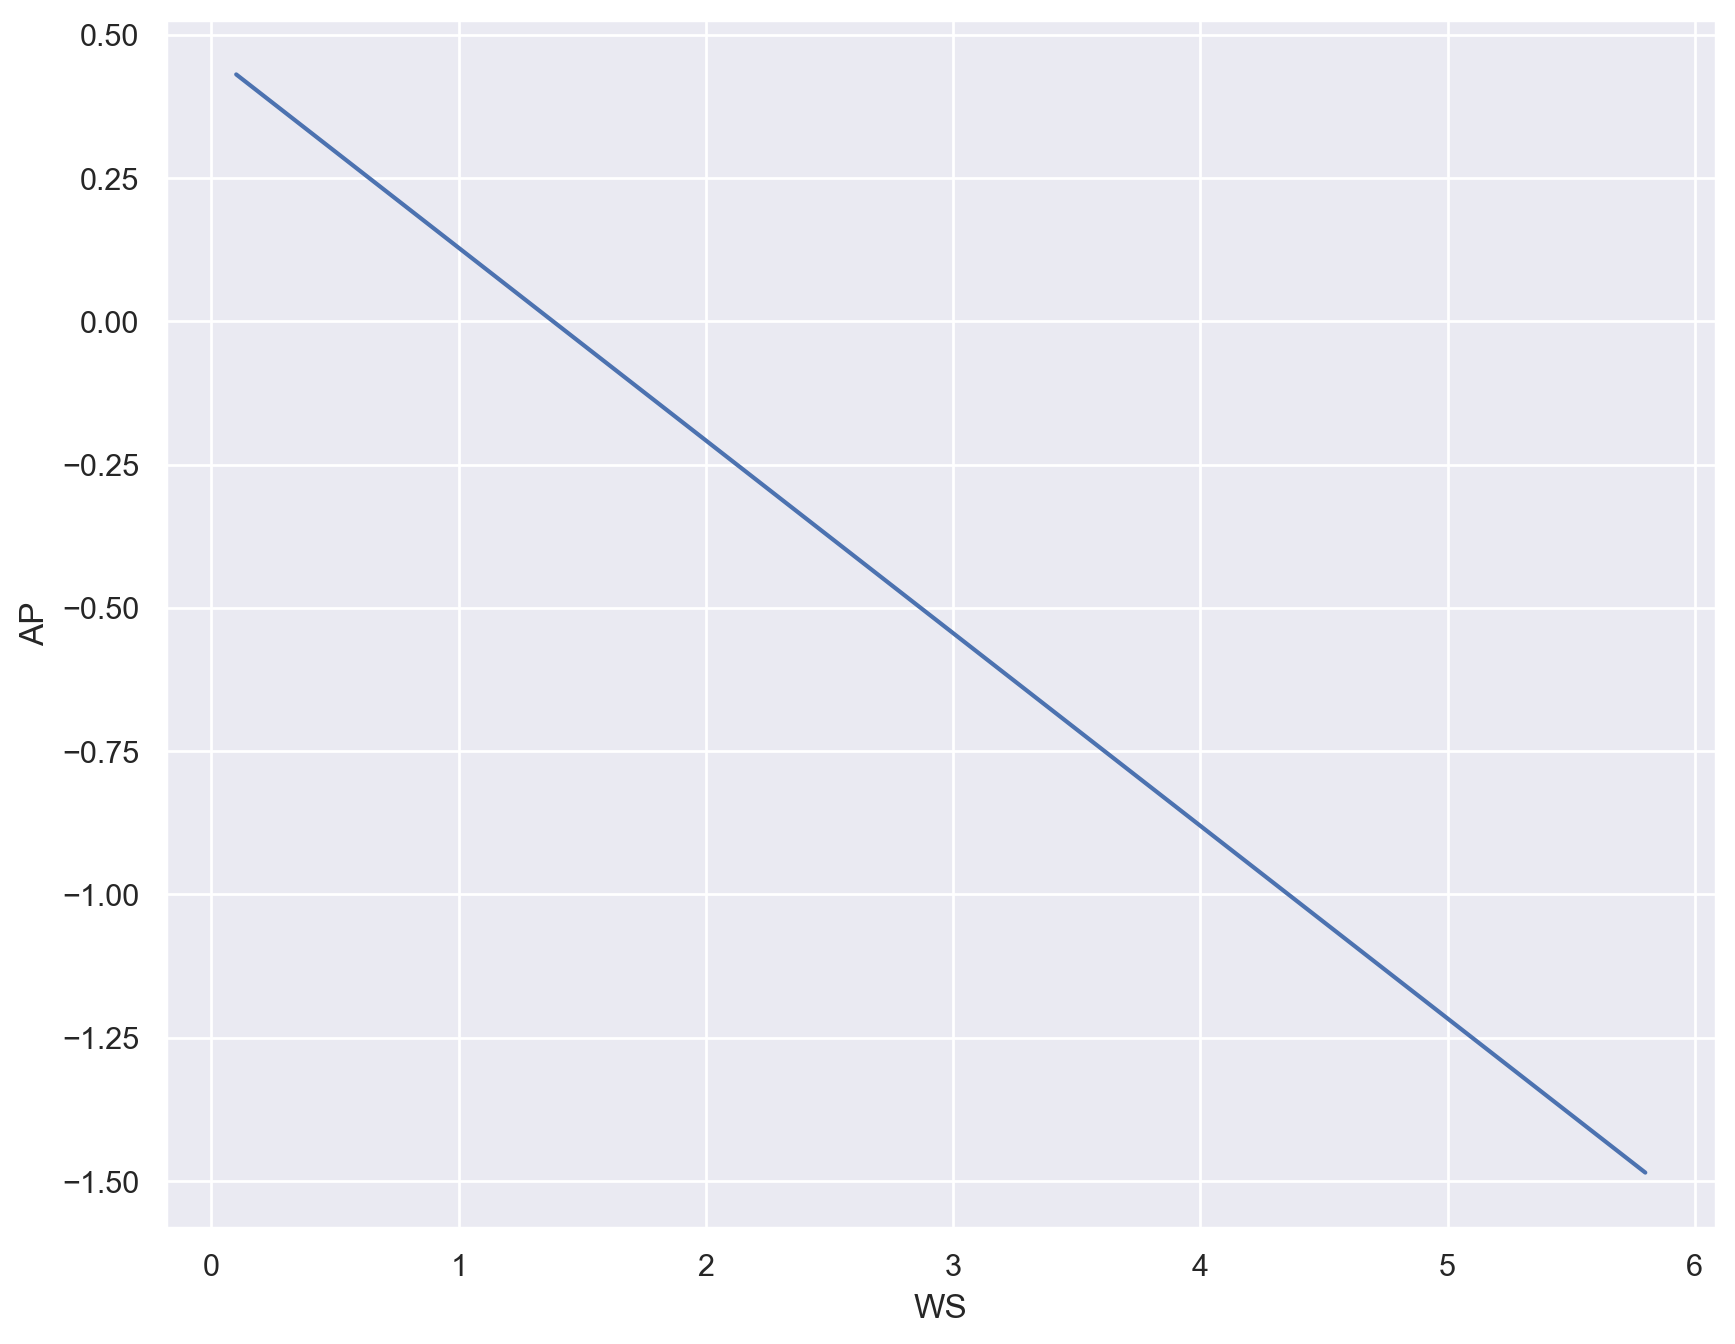
\includegraphics[width=.7\textwidth]{figures//fig_WS_fit.png}
	\caption{变量AP与风速变量WS的拟合曲线}
	\label{fig3-6}
\end{figure}

从图\ref{fig3-6}中可以看出,根据拟合的图像,随着变量WS的上升,因变量AP不断下降且AP的变化范围较显著,因此将变量WS(即风速变量)列入“有较为显著的单向影响因素”类别。

同理,为了行文的简略。对之后的变量,直接使用拟合图描述因变量AP随自变量的变化过程

\ding{173} 可视化统计AP变量与温度变量T之间的关系:

对AP与T的关系进行拟合,如图\ref{fig3-7}所示:
\begin{figure}[!h]
	\centering
	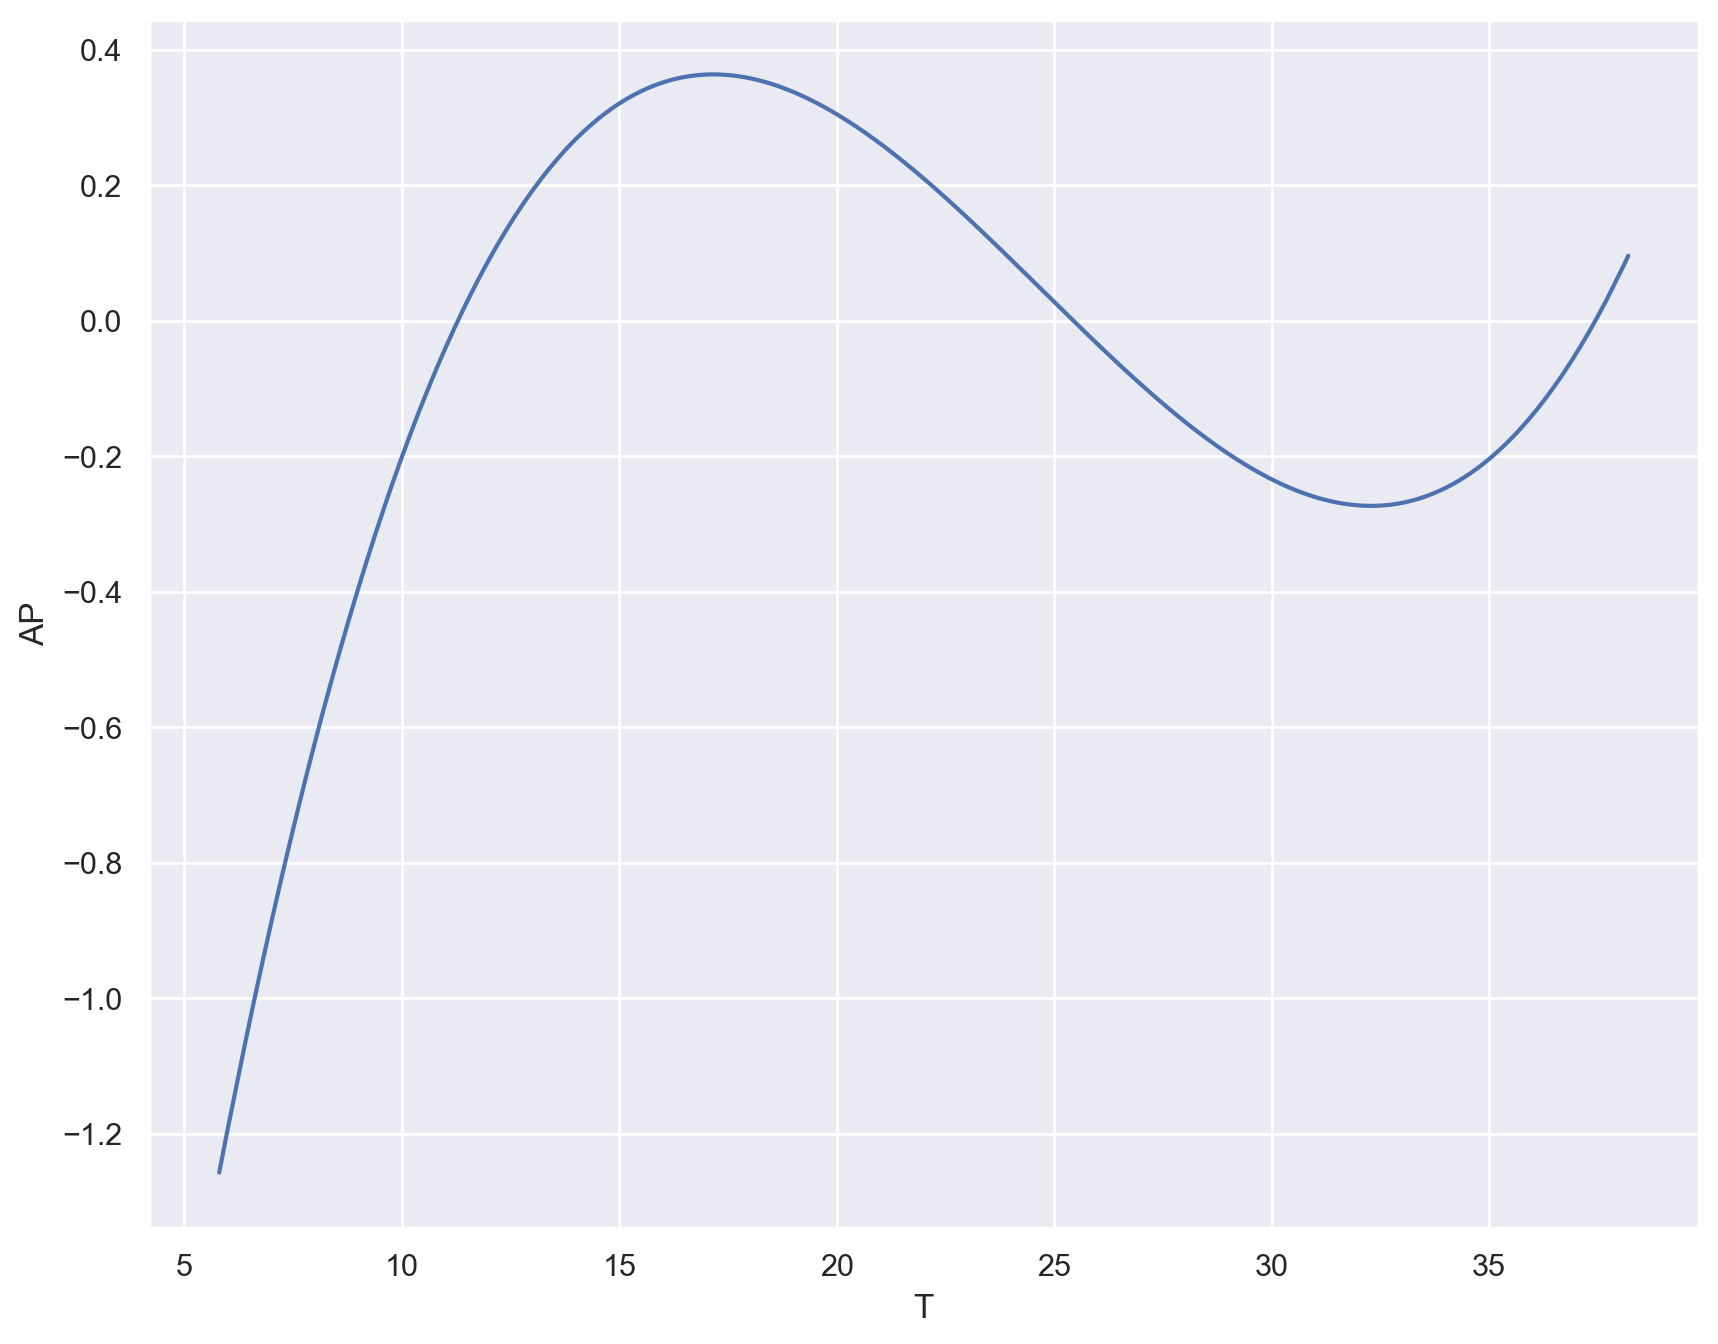
\includegraphics[width=.7\textwidth]{figures//fig_T_fit.png}
	\caption{变量AP与温度变量T的拟合曲线}
	\label{fig3-7}
\end{figure}

如图\ref{fig3-7}所示,在T处于5℃-17℃时,随着T的上升,AP不断上升;当T处于17℃-32℃时,随着T上升AP不断下降;当T处于32℃以上时,随着T的上升,AP再一次上升。AP的变化范围较显著,因此将温度变量T列为“有显著的双向影响因素”类别。

\ding{174} 可视化统计AP变量与湿度变量H之间的关系:

对AP与H的关系进行拟合,如图\ref{fig3-8}所示:
\begin{figure}[!h]
	\centering
	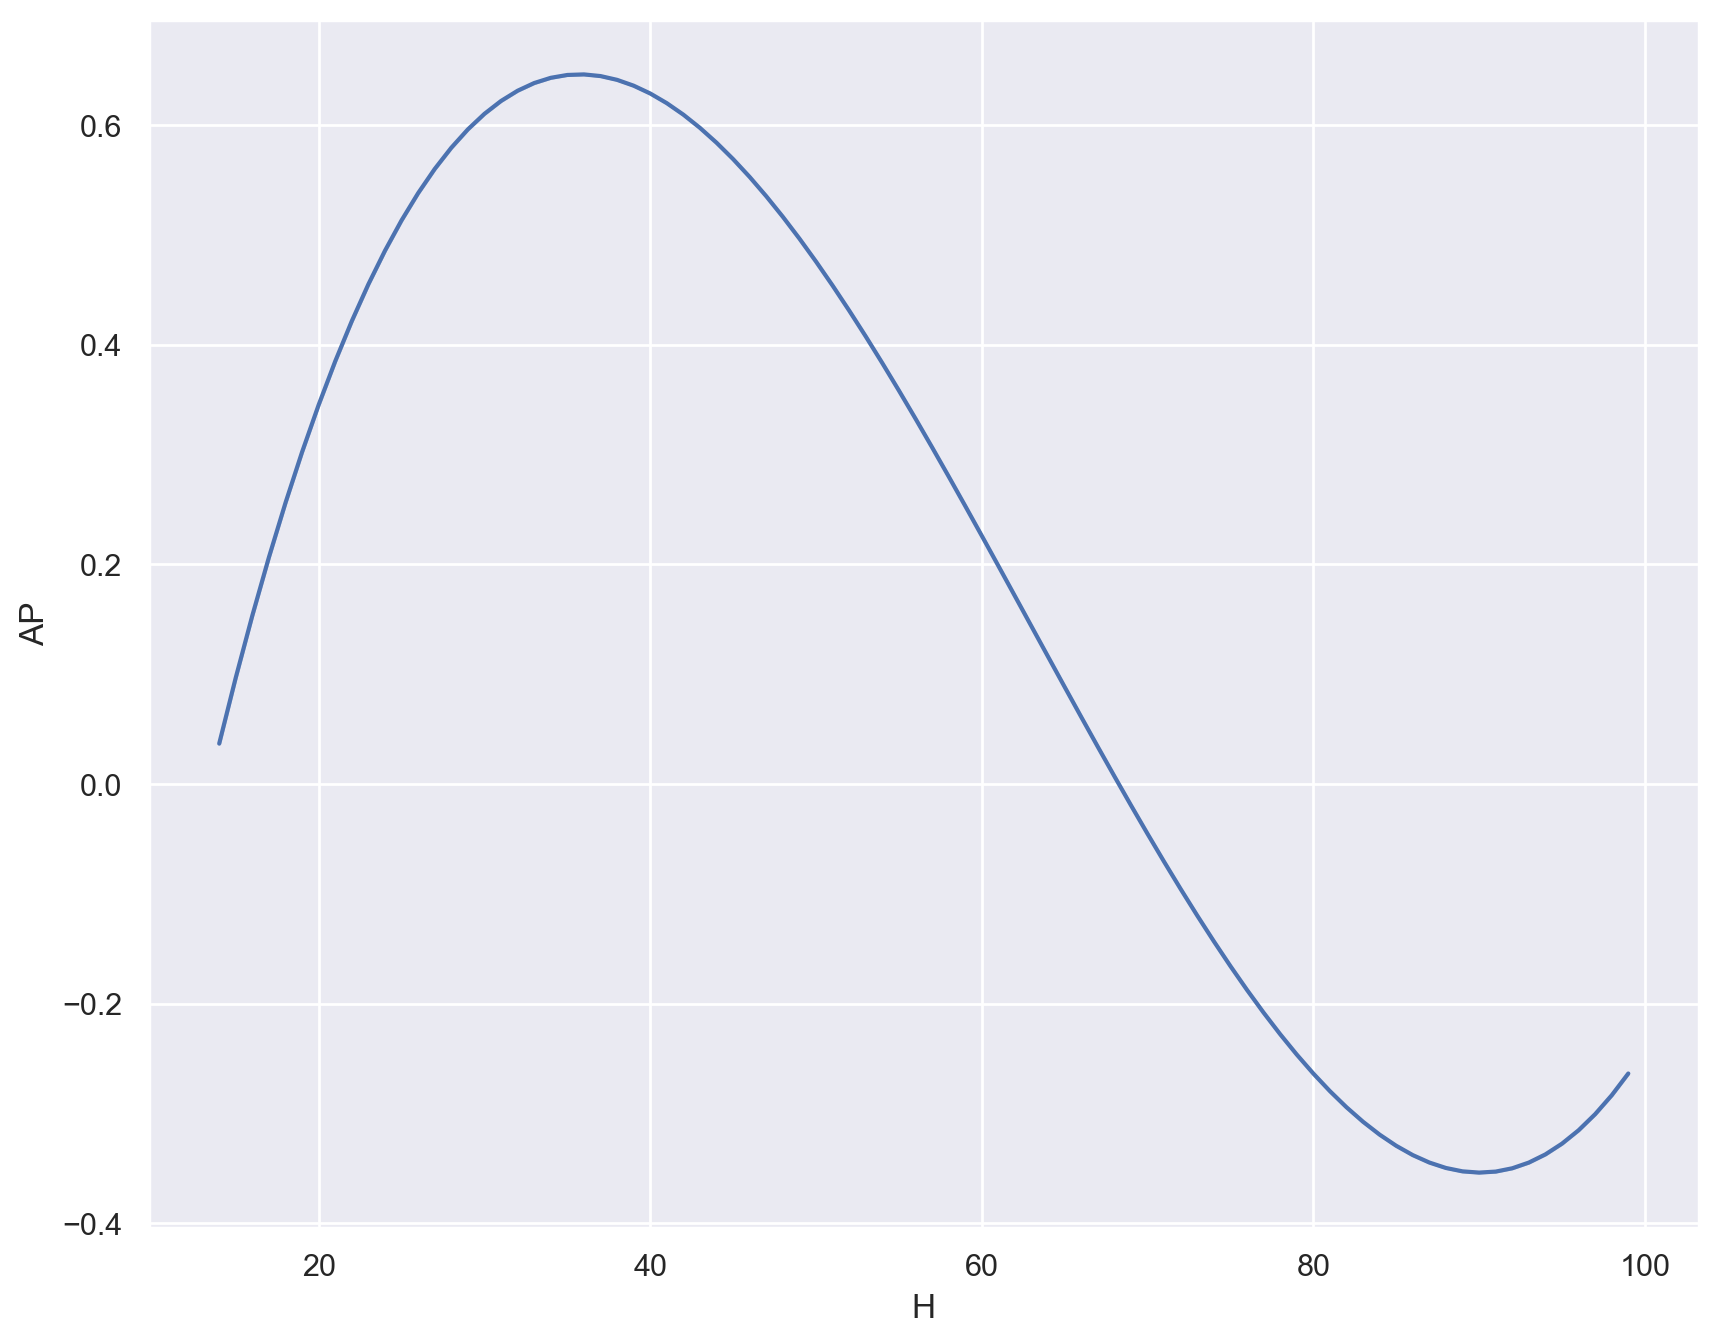
\includegraphics[width=.7\textwidth]{figures//fig_H_fit.png}
	\caption{变量AP与湿度变量H的拟合曲线}
	\label{fig3-8}
\end{figure}

如图\ref{fig3-8}所示,在H处于10\%-35\%区间内,随着H的上升,变量AP不断上升;在H处于35\%-88\%区间,随着H的上升,变量AP不断下降;对于H处于88\%以上的数据,虽然在图中有一点略微的凸起,但是可以认为是模型的误差。以及AP的变化范围较为显著。因此将湿度变量H列入“有较为显著的双向影响因素”类别

\ding{174} 可视化统计AP变量与气压变量P之间的关系:

对AP与P的关系进行拟合,如图\ref{fig3-9}所示:
\begin{figure}[!h]
	\centering
	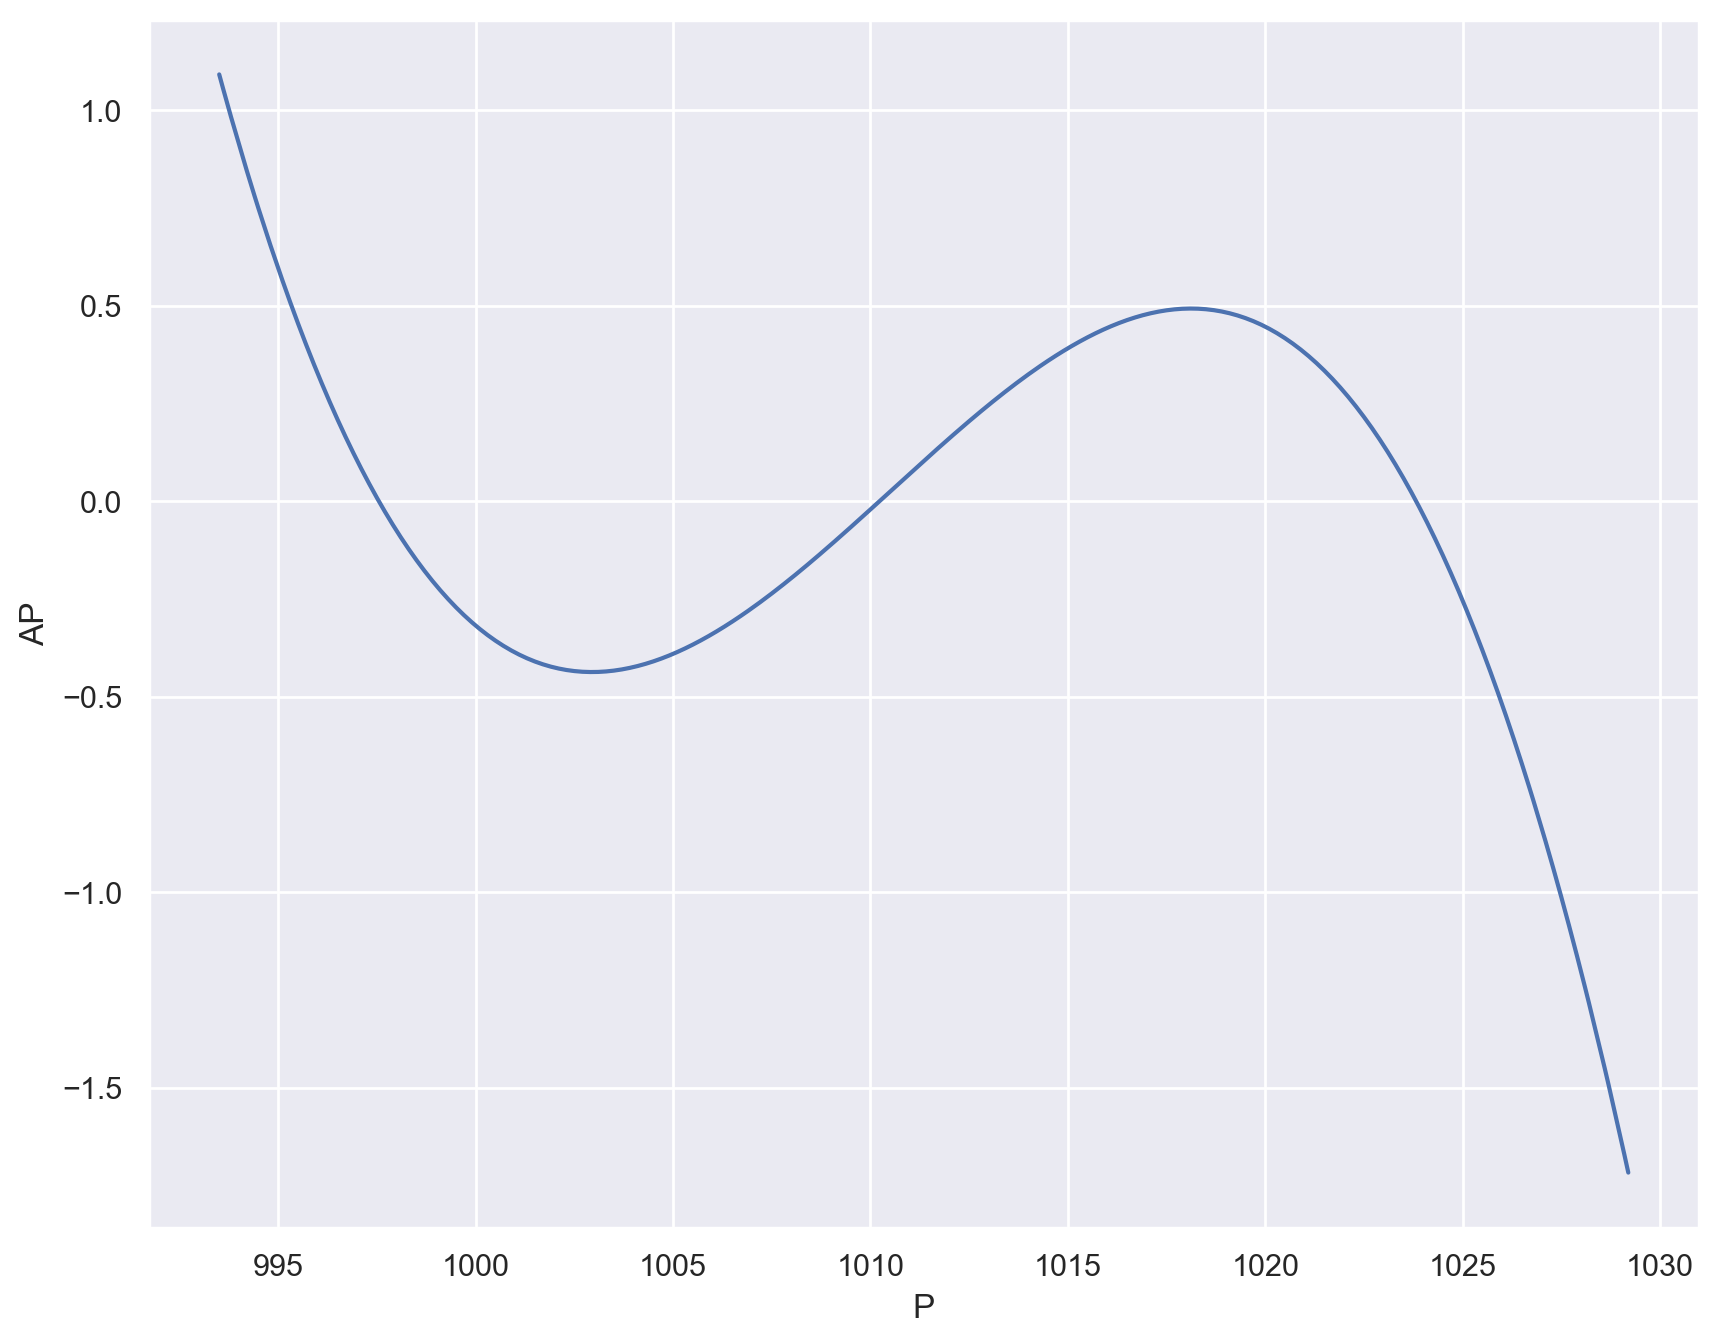
\includegraphics[width=.7\textwidth]{figures//fig_P_fit.png}
	\caption{变量AP与气压变量P的拟合曲线}
	\label{fig3-9}
\end{figure}

如图\ref{fig3-9}所示,在P处于995MPa到1003MPa之间时,随着P的上升,变量AP不断下降;在P处于1003MPa到1018MPa之间时,随着P的上升,变量AP不断上升;在P大于1018MPa时,随着P的上升,变量AP不断下降。且变量AP的变化范围较为显著。因此将气压变量P列入“有较为显著的双向影响因素”类别

\ding{175} 可视化统计AP变量与风向变量WD之间的关系:

对AP与WD的关系进行拟合,如图\ref{fig3-10}所示:
\begin{figure}[!h]
	\centering
	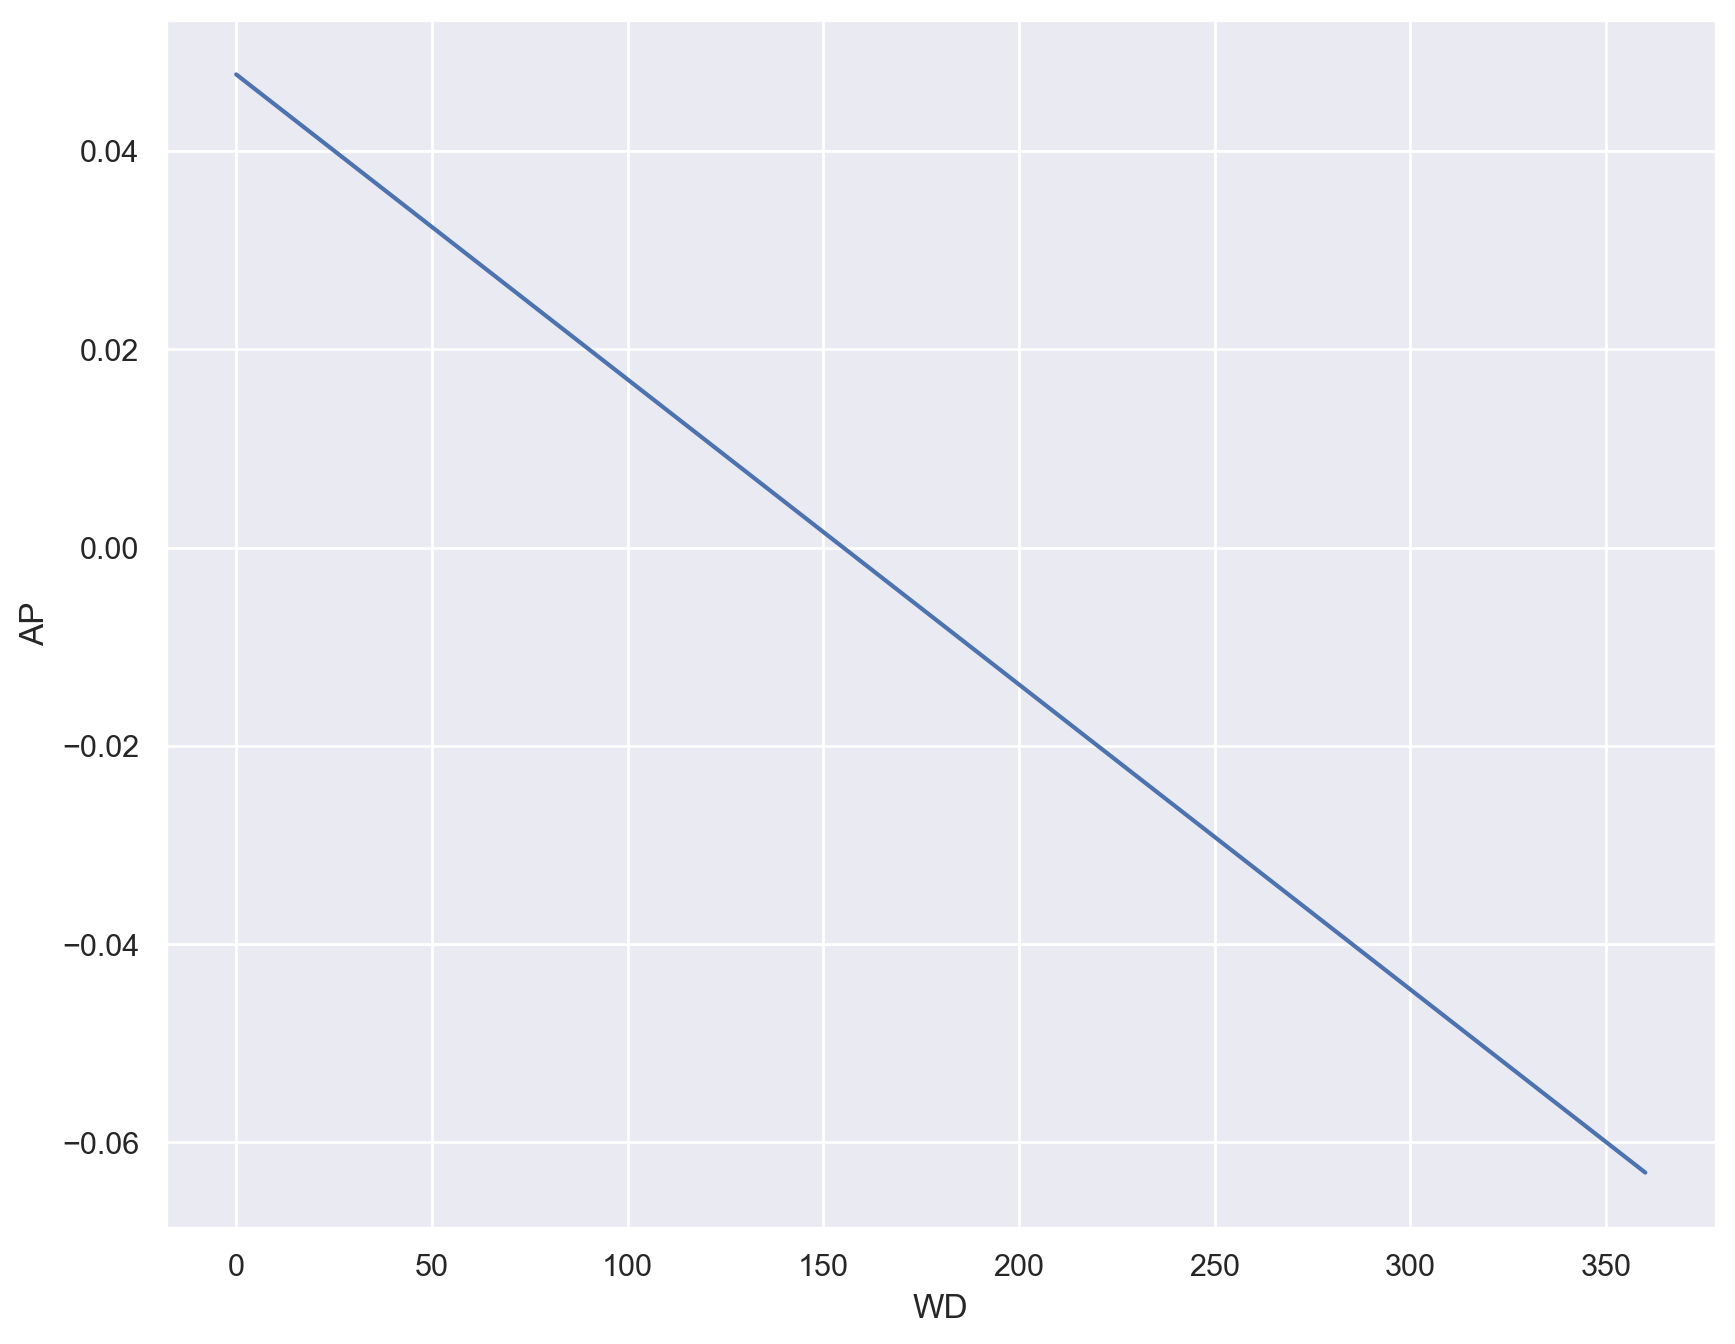
\includegraphics[width=.7\textwidth]{figures//fig_WD_fit.png}
	\caption{变量AP与风向变量WD的拟合曲线}
	\label{fig3-10}
\end{figure}

如图\ref{fig3-10}所示,随着WD的增加,变量AP的变化范围并不显著,仅在0.04到-0.06这个区间变化。因此将风向变量WD列入“无显著影响因素”类别。

\subsubsection{模型结果归纳}
最终,我们将5种气象条件分为以下三类:有较为显著的单向影响类别,有较为显著的双向影响类别,无显著影响类别。通过自定义变量AP用于标志所有的污染物对环境影响的恶劣程度。此处,对各个类别的解释如下:

(1)有较显著单向影响类:在定义域全区间内,随着变量值的上升,变量AP的取值不断上升或下降。也即在全定义域区间内都为正相关或负相关。

(2)有较为显著的双向影响类别:存在被定义域包含的部分区间P内,随着变量值的上升,变量AP的取值不断上升;存在被定义域包含的部分区间Q,随着变量值的上升,变量AP的取值不断下降。也即在部分区间内为正相关,部分区间内为负相关。

(3)无显著影响类别:在定义域全区间内,随着变量值的上升,变量AP的值没有显著的变化。

5种气象类型的分类结果如表所示:
\begin{table}[h!]
	\caption{气象类型分类表}\label{tab:table4-6}
	\begin{center}
		\begin{tabular}{|c|c|}
			\hline
			类型名&变量\\
			\hline
			有显著的单向影响因素&风速变量WS\\
			\hline
			有显著的双向影响因素&温度变量T,比湿变量H,气压变量P\\
			\hline
			无显著影响因素&风向变量WD\\
			\hline
		\end{tabular}
	\end{center}
\end{table}


\subsection{问题三:依据一次预报数据和实测数据建立二次预报模型}
\subsubsection{问题描述和分析}
WRF-CMAQ预报模型由于自身原因和来自不完全明晰臭氧等污染物生成机理的外因,导致其预报的结果并不理想。因此题目要求我们结合一次预报数据和实测数据建立二次预报模型进行更准确的污染物浓度预测。问题三要求我们建立一个同时适用于监测点A,B和C的二次预报模型(不考虑监测点间影响),并给出更加精确的首要污染物预测,并且要求AQI预测值的最大相对误差尽量小。

考虑到这个问题是通过由过去若干个时刻的状态推测未来时刻的状态,我们想要通过LSTM对历史的特征进行学习,以此来修正一次模型预测的数据,最后达到提升预测准确度的目的。我们了解到,在对空气质量预报领域主要有2种类型的模型,一种是数值模型,如WRF-CMAQ是通过对气象场的模拟从而进行预测,另外一类则是统计模型,典型的如神经网络和多元回归等模型。这两类模型各有优缺点,从题目中我们看到了数值模型的局限性,因此我们选择建立一个统计模型,并采用预训练和微调两阶段,在第二阶段与WRF-CMAQ的一次预报数据结合进行微调,从而取长补短。

如前所述,我们的思路是将数值模型与统计模型结合,也就是将由WRF-CMAQ运行的一次预报数据和我们训练的基于LSTM的统计模型结合。因此我们建立的二次模型分为两个阶段,在第一阶段的预训练过程中,完全使用监测点逐小时实测的污染物浓度和气象条件数据训练一个LSTM模型,在第二阶段微调的时候,再将一次预报数据引入和用LSTM模型预测的数据经过SVM输出最终的预测结果。
\subsubsection{数据预处理}
由于我们使用的LSTM对时间序列的逐小时顺序要求,并且还要考虑在第二阶段与一次预报数据结合时候的对齐问题,我们在进行模型的构建之前,对提供的数据进行了非常严格的预处理:
\begin{itemize}
	\item 填补缺失/无效数据。我们首先用pandas把数据转化成pandas DataFrame,然后进行Exploratory Data Analasis(EDA)。通过pandas使得我们能够快速对数据整体结构有一个快速清晰的认知,并且能够对数据进行快速的操作。由于LSTM对时间连续性的需求,我们会尽可能用插值法填补中间缺失的数据,对于有多行的缺失并且在时间序列前端的数据,如A监测点的2019年4月逐小时实测数据有100多行缺失,我们选择直接从5月开始进行输入。
	\item 数据清洗。除了缺失/无效数据外,我们还理应检查数据是否有异常值,我们首先由profile_report对所有变量进行频率分别可视化,并生成每个变量的细节报告,然后搜寻可能的异常值,对于异常值的判断,除了浓度值小于0的数据以外,根据题目所给的空气质量分指数及对应污染物浓度限值表中的浓度限值,我们可以将每个浓度按照大小归到其中一个区间,由此我们假设所有"跨区"数据为异常数据,即如果有非常少的数据所在区间的前一个区间没有该类中的其他数据存在,我们就认为该数据为异常数据,并根据时间序列选择使用前后插值,或前一刻数据进行代替。
	\item 核对数据类型。数据类型的正确与否直接关系到后面对数据的运算,因此在正式运用数据之前需要确保每一个变量的数据类型是正确的。
\end{itemize}
\subsubsection{模型建立与求解}
\begin{figure}[!h]
	\centering
	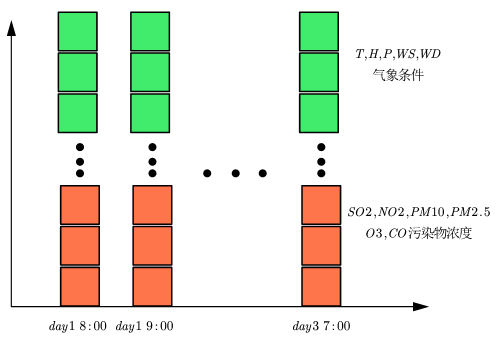
\includegraphics[width=.7\textwidth]{LSTM_input.png}
	\caption{LSTM模型输入。我们按图中所示的方式把三天(72小时)的实测数据输入到LSTM模型中进行训练。}
	\label{LSTM-INPUT}
\end{figure}
我们先运用LSTM对实际的污染物浓度(6种)+气象条件(5种)按照每三天(72小时实测数据)一次,进行训练,随后把一次模型预测的数据(11种)按三天取平均。例如:2020年7月23号的模型预测23,24和25号的11种数据取平均后做为一次模型2020-07-23的预测值。在确保预测数据和实测数据的日期一致后,如图所示,把经过预处理的预测数据接入到已经用实测数据训练好的LSTM模型里,最后直接输出18个数据,每6个为一天的预测污染物浓度。

\begin{figure}
	\centering
	\begin{subfigure}[ht]{.4\textwidth}
		\centering
		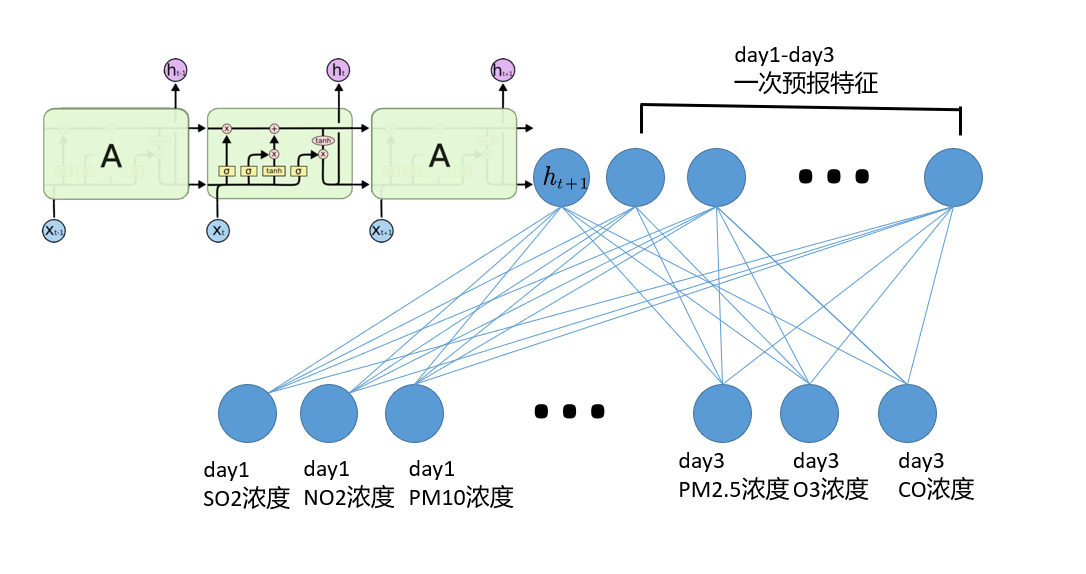
\includegraphics[width=\textwidth]{model.jpg}
	\end{subfigure}
	\begin{subfigure}[ht]{.4\textwidth}
		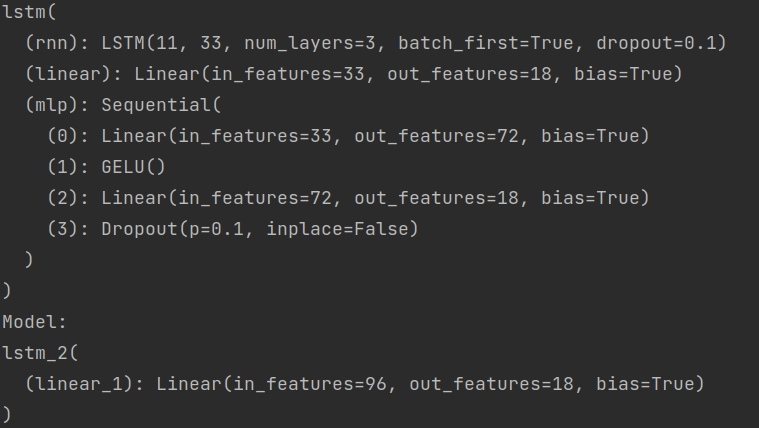
\includegraphics[width=\textwidth]{figures/model_2.jpg}
	\end{subfigure}
	\caption{二次预测模型。通过LSTM对实测数据进行学习后接入一次模型预测的数据来提升预测准确度。最后直接输出三天的污染物浓度。}
	\label{model}
\end{figure}

\begin{table}[h!]
	\caption{污染物浓度及AQI预测结果}\label{tab: AQI_Pre}
	\begin{center}
	\resizebox{.95\columnwidth}{!}{
		\begin{tabular}{|c|c|c|c|c|c|c|c|c|c|}
			\hline
			\multirow{2}{*}{预报日期}&\multirow{2}{*}{地点}&\multicolumn{8}{|c|}{二次模型日值预测} \\
			\cline{3-10}
			& &SO2(μg/m³)&NO2(μg/m³)&PM10(μg/m³)&PM2.5(μg/m³)&O3最大八小时滑动平均(μg/m³)&CO(mg/m³)&AQI&首要污染物\\
			\hline
			2020/7/13&监测点A&6.06&43.60&41.28&35.92&86.76&0.73&55&NO2\\
			\hline
			2020/7/14&监测点A&7.90&41.13&53.02&22.39&46.77&0.61&52&NO2\&PM10\\
			\hline
			2020/7/15&监测点A&9.80&42.16&54.02&48.52&48.61&1.10&67&PM2.5\\
			\hline
			2020/7/13&监测点B&2.09&38.69&92.57&11.58&106.18&0.52&72&PM10\\
			\hline
			2020/7/14&监测点B&21.52&19.93&41.09&16.18&49.90&0.53&42&PM10\\
			\hline
			2020/7/15&监测点B&13.48&27.40&64.16&19.99&23.26&0.47&58&PM10\\
			\hline
			2020/7/13&监测点C&9.03&31.59&72.48&17.95&-1.87&0.82&62&PM10\\
			\hline
			2020/7/14&监测点C&9.12&40.59&49.47&30.22&49.57&1.03&51&NO2\\
			\hline
			2020/7/15&监测点C&4.62&16.72&50.68&15.79&20.01&0.80&51&PM10\\
			\hline
		\end{tabular}
	}
	\end{center}
\end{table}
\subsection{问题四:建立区域协同模型提高预测精度}
\subsubsection{问题描述和分析}
问题四与问题三大致相同,但区别是问题四要求考虑到区域之间的互相影响,建立一个区域协同模型进行预测。因为相邻区域之间的污染物通常具有相关性,因此通过建立一个多区域的协同模型能够提高预测精度。考虑到区域之间的协同预报作用,我们选择将4个监测点的实测与一次预报同时输入到我们问题三中建立的模型进行预测,但这也产生了新的问题,同时将4个监测点的数据输入就意味着整个模型的参数规模也变为了原来的4倍,模型也变得更为复杂,而这并不是我们希望的,因此我们首先需要进行降维再输入到问题三中的模型。考虑到4个监测点的气象条件共同的对其他监测点进行影响,我们认为同一个监测点的数据是符合参数共享条件的,也就是说我们可以使用卷积操作实现降维操作。

在预训练阶段,我们使用了72个4×1卷积核的滤波器使得时间序列从72×4×11维重新降维到问题三中的72×11维,而在微调阶段也同样使用4×1的卷积核进行降维,达到问题三的规模,在问题四中,我们对四个监测点分别训练各自的模型,每次的输入都是一样的,只是每次训练所用的标签分别是每个监测点的实测浓度,因此每次的卷积核是不同的,我们认为卷积起到了调节各个监测点彼此影响程度的作用。
\subsubsection{数据预处理}
我们利用附件1和3中,监测点A,A1,A2和A3的一次模型预测数据和实测数据进行协同训练。与问题三一样,同样面临严格的数据预处理要求,而且我们发现相比问题三的B和C监测点:
\begin{itemize}
	\item 填补缺失/无效数据。我们首先用pandas把数据转化成pandas DataFrame,然后进行Exploratory Data Analasis(EDA)。通过pandas使得我们能够快速对数据整体结构有一个快速清晰的认知,并且能够对数据进行快速的操作。由于LSTM对时间连续性的需求,我们会尽可能用插值法填补中间缺失的数据,对于有多行的缺失并且在时间序列前端的数据,如A监测点的2019年4月逐小时实测数据有100多行缺失,我们选择直接从5月开始进行输入。
	\item 数据清洗。除了缺失/无效数据外,我们还理应检查数据是否有异常值,我们首先由profile_report对所有变量进行频率分别可视化,并生成每个变量的细节报告,然后搜寻可能的异常值,对于异常值的判断,除了浓度值小于0的数据以外,根据题目所给的空气质量分指数及对应污染物浓度限值表中的浓度限值,我们可以将每个浓度按照大小归到其中一个区间,由此我们假设所有"跨区"数据为异常数据,即如果有非常少的数据所在区间的前一个区间没有该类中的其他数据存在,我们就认为该数据为异常数据,并根据时间序列选择使用前后插值,或前一刻数据进行代替。
	\item 核对数据类型。数据类型的正确与否直接关系到后面对数据的运算,因此在正式运用数据之前需要确保每一个变量的数据类型是正确的。
\end{itemize}

\subsubsection{模型建立与求解}
我们在问题三的基础上加上了A1-A3三个监测点的小时级实测数据与监测点A的小时级实测数据一并放到LSTM中进行模型的预训练,然后再把四个监测点的一次模型预测数据连接到LSTM上,再加上一个4X1的卷积核进行降维,最后输出72个神经元,分别作为4个监测点3天的六种污染物浓度。\\
相对于AQI的相对误差,我们选择MSE作为我们的判别依据,我们的模型所给出的AQI的MSE为897.87,一次模型给出的AQI的MSE为1682.42,对于各污染物浓度的MSE如表\ref{tab:pol_mse}所示:
\begin{table}
	\caption{各污染物浓度MSE}\label{tab:pol_mse}
	\begin{center}
	\resizebox{.95\columnwidth}{!}{
		\begin{tabular}[ht]{|c|c|c|c|c|c|c|}
			\hline
			模型 & SO2($\mu g/m^3$) & NO2($\mu g/m^3$) & PM10($\mu g/m^3$) & PM2.5($\mu g/m^3$) & O3($\mu g/m^3$) & CO($\mu g/m^3$)\\
			\hline
			一次模型 & 21.41 & 2221.62 & 2105.39 & 1135.74 & 2728.31 & 0.32\\
			\hline
			二次模型 & 13.21 & 584.92 & 705.37 & 629.26 & 1828.01 & 0.16\\
			\hline
		\end{tabular}
	}
	\end{center}
\end{table}
\section{模型的评价}
\subsection{模型的优点}
我们的模型可以从实测历史数据中不断学习,大大提高了臭氧(O3)的预测准确度,进而提升了AQI及主要污染物的预测精度。除此之外,我们的模型易于训练,可扩展性强,能够泛化到不同的问题上。在问题三中,我们预测的不同监测点的AQI的精确度平均提升了接近2倍,对臭氧的预测准确度提升了近10倍。\\
从图\ref{model_loss}中可以看出模型在不同的监测点下都能很好的收敛,说明我们的模型的泛化程度很高,能够很好的应对不同监测点的情况。
\begin{figure}
	\centering
	\begin{subfigure}[ht]{.3\textwidth}
		\centering
		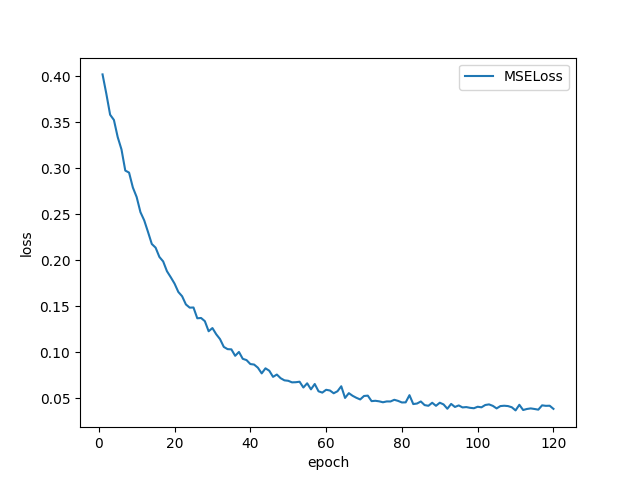
\includegraphics[width=\textwidth]{figures/model_loss.png}
		\caption{监测点A模型LOSS}
		\label{A_model_loss}
	\end{subfigure}
	\begin{subfigure}[ht]{.3\textwidth}
		\centering
		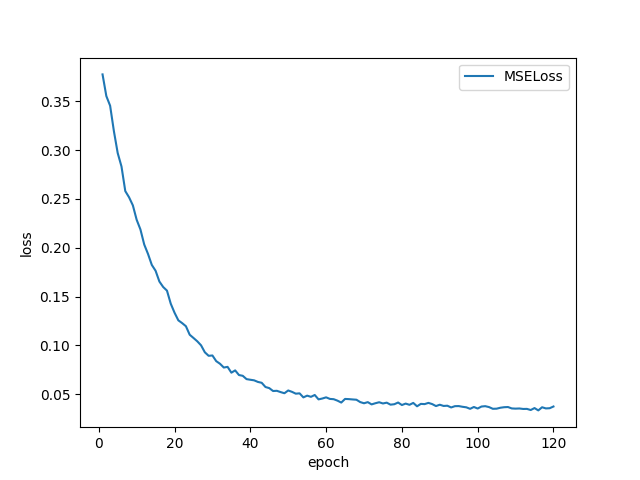
\includegraphics[width=\textwidth]{figures/model_loss_B.png}
		\caption{监测点B模型LOSS}
		\label{B_model_loss}
	\end{subfigure}
	\begin{subfigure}[ht]{.3\textwidth}
		\centering
		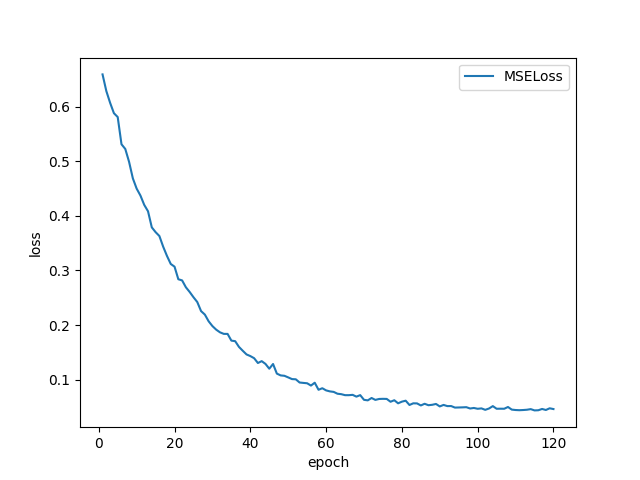
\includegraphics[width=\textwidth]{figures/Model_loss_C.png}
		\caption{监测点C模型LOSS}
		\label{C_model_loss}
	\end{subfigure}
	\caption{不同监测点的Model Loss}
	\label{model_loss}
\end{figure}

\begin{table}
	\begin{center}
		\resizebox{.95\columnwidth}{!}{
			\begin{tabular}[hb]{|c|c|c|}
				\hline
				模型(监测地点) & AQI & 主要污染物 \\
				\hline
				一次模型(A) & 1682.42 & 24\%\\
				\hline
				二次模型(A) & 897.86 & 26\%\\
				\hline
				二次模型(B) & 612.49 & 39\%\\
				\hline
				二次模型(C) & 217.69 & 33\%\\
				\hline
			\end{tabular}
		}
	\end{center}
	\caption{各监测点AQI的MSE及主要污染物的预测正确率。}\label{tab:pos_AQI}
\end{table}
从表\ref{tab:pol_mse}和表\ref{tab:pos_AQI}中可以看出,我们的模型在对各污染物浓度的预测中有一个2-4倍的提升,在对各监测点的AQI的预测中有极大的提升,并且在对主要污染物的预测正确率上也有较大的提高。
\subsection{模型的缺点}
\begin{itemize}
	\item 对于PM2.5和PM10的估计误差较大。
	\item 模型对数据格式要求比较严格,只能读入连续的数据,并且要求不同检测地点的数据要同步。
\end{itemize}



% \section{写作参考格式}
% 写作过程中可能要用到一些格式参考,正式写作的时候,可以直接将这一章删掉即可。

% \textbf{无序列表格式}
% \begin{itemize}
% \item 无序列表1
% \item 无序列表2
% \item 无序列表3
% \item 无序列表4
% \end{itemize}


% \textbf{表格格式}

% \begin{tabular}{cc}
%  \hline
%  \makebox[0.4\textwidth][c]{符号}	&  \makebox[0.5\textwidth][c]{意义} \\ \hline
%  D	    & 宽度(cm) \\ \hline
%  L	    & 长度(cm)  \\ \hline
% \end{tabular}


%
%\textbf{图片格式}
%\begin{figure}[h]
%\centering
%\includegraphics[width=5cm]{xxx.jpg}
%\caption{图片标题}
%\end{figure}

\section{参考文献}
%参考文献
\begin{thebibliography}{1.2}%宽度9
\setlength{\itemsep}{-2mm}
 \bibitem{ref1}
 宋鹏程, 张馨文, 黄强, 等. 我国城市环境空气质量预报主要模型及应用[J]. 四川环境, 2019, 3.
 \bibitem{ref2}
 伯鑫 等. 空气质量模型(SMOKE、WRF、CMAQ等)操作指南及案例研究 [M]. 北京: 中国环境出版集团, 2019.
 \bibitem{ref3}
 戴树桂. 环境化学 [M]. 北京: 高等教育出版社, 1997.
 \bibitem{ref4}
 赵秋月, 李荔, 李慧鹏. 国内外近地面臭氧污染研究进展 [J]. 环境科技, 2018, 31(05): 72-76.
 \bibitem{ref5}
 陈敏东. 大气臭氧污染形成机制及研究进展 [J/OL] 2018, https://max.book118.com/html/2018/0201/151478594.shtm. 
\end{thebibliography}

\newpage
%附录
\appendix
\section{程序代码}
%设置不同语言即可。
\begin{lstlisting}[language=Matlab] 
kk=2;[mdd,ndd]=size(dd);
while ~isempty(V)
[tmpd,j]=min(W(i,V));tmpj=V(j);
for k=2:ndd
[tmp1,jj]=min(dd(1,k)+W(dd(2,k),V));
tmp2=V(jj);tt(k-1,:)=[tmp1,tmp2,jj];
end
tmp=[tmpd,tmpj,j;tt];[tmp3,tmp4]=min(tmp(:,1));
if tmp3==tmpd, ss(1:2,kk)=[i;tmp(tmp4,2)];
else,tmp5=find(ss(:,tmp4)~=0);tmp6=length(tmp5);
if dd(2,tmp4)==ss(tmp6,tmp4)
ss(1:tmp6+1,kk)=[ss(tmp5,tmp4);tmp(tmp4,2)];
else, ss(1:3,kk)=[i;dd(2,tmp4);tmp(tmp4,2)];
end;end
dd=[dd,[tmp3;tmp(tmp4,2)]];V(tmp(tmp4,3))=[];
[mdd,ndd]=size(dd);kk=kk+1;
end; S=ss; D=dd(1,:);
 \end{lstlisting}


\end{document} 